\documentclass[12pt,a4paper]{article}

% Essential packages
\usepackage[utf8]{inputenc}
\usepackage[margin=2.5cm]{geometry}
\usepackage{graphicx}
\usepackage{float}
\usepackage[hidelinks]{hyperref}
\usepackage{booktabs}
\usepackage{pgfplots}
\usepackage{appendix}

% Document title and author information
\title{\textbf{Enhancing DAEN Program Effectiveness: Analysis of Alumni Interview Feedback at George Mason University}}
\author{Lingyun Dai, James Baldo}
\date{\today}

\begin{document}

\maketitle

% Abstract
\begin{abstract}
The effectiveness of the DAEN program at George 
Mason University is critical as the department aim to provide industry-relevant education, focusing on tools, technologies, and skills that are directly applicable in professional roles. This study presents analysis of the DAEN program at the College of Computing and Engineering at George Mason University, examining industry demands and program effectiveness through comprehensive alumni feedback. The research is conducted through alumni interviews. The interviews are designed with structured qualitative and quantitative questions to evaluate various aspects of program alumni including academic profile, employment trajectories, technical skill utilization in jobs, program technical skill utilization, and program feedback. Data was collected through anonymous interview recordings in either audio or text format based on the interview platform used. Audio interview recordings were processed confidentially using AWS transcribe to generate text transcripts. The text transcripts were cleaned and extracted into columns in a CSV file using local natural language processing toolkit. The data was visualized using Tableau to identify patterns in employment outcomes, 
skill utilization, and areas for program enhancement. The data visualizations provide actionable insights for curriculum development 
and program improvements, while also offering valuable metrics for 
assessing the program's effectiveness in preparing graduates for 
industry demands. This research contributes to the broader 
understanding of DAEN program effectiveness.

\textbf{Keywords:} DAEN, Alumni, Employment, Program, Data,
 Analysis, Skill, Interview, Industry
\end{abstract}

\newpage
\tableofcontents
\newpage

\section*{List of Abbreviations}
\begin{tabular}{ll}
DAEN & Data Analytics Engineering\\
AWS & Amazon Web Services\\
M.S. & Master of Science\\
NLP & Natural Language Processing\\
MS & Microsoft\\
\end{tabular}
\newpage

% 1. Introduction Section
\section{Introduction}
\subsection{Purpose}
The primary objective of this research is to evaluate the DAEN 
program's effectiveness through comprehensive alumni interviews. Through structured feedback 
obtained from program alumni, this study conducts a 
detailed analysis of employment outcomes and program performance 
metrics. These insights are instrumental in enabling the DAEN 
department to implement strategic enhancements to the program's curriculum development and technology integration.

\subsection{Readership}
The report is intended for the DAEN program academic and 
administrative personnel including leaderships, stackholders, 
and development team. The findings presented in this report will provide valuable insights for improving program effectiveness, curriculum design, and student outcomes.

\subsection{Doc Structure}
This report is organized into seven main sections. The Introduction 
establishes the research context and objectives. The Problem 
Statement formulates the research questions and scope. 
The Data section outlines the interview-based data collection 
methodology, data processing methodology, data quality interpretation, and interview question design. The Analysis section details the data 
processing pipeline and techniques employed. The Visualization section presents the derived data visualizations 
and their interpretations. The Findings section synthesizes key 
insights obtained through visualizations. Finally, the Next 
Steps and Lessons Learned section proposes future research 
directions and methodological improvements.

% 2. Problem Statement Section
\section{Problem Statement}
\subsection{Alumni Feedback}
There are 14 alumni participated in the interview who graduated between year of 2019 and 2023. From the 14 alumni interviewed, the average program rating is 3.7 out of 5, the average number of jobs held after graduation is 2 jobs. Data Analyst emerges as the most prevalent job title. The most frequently used technologies are python and SQL, the most frequently used cloud platform is AWS, the most used tools are Power BI and Tableau. The common area for program improvement reported by the 14 alumni are more hands-on projects, cloud, and practical application. 


\subsection{Focus}
The study aims to evaluate the gap between the most used skills in alumni career and the most valuable skills acquired in the program. The study also aims to identify the areas for program improvement and how well the program prepared alumni for their career.

\subsection{Problem}
The DAEN program faces significant challenges in evaluating program effectiveness as this represents the first systematic effort to gather alumni feedback. The absence of a centralized alumni database and limited alumni engagement mechanisms make it difficult to reach and collect comprehensive feedback from program graduates. After the alumni feedback was gathered and processed, some key problems with the program was discovered. First, the data reveals that while most alumni work with cloud platforms in their current roles, many received limited exposure to cloud technologies during their coursework. Second, there is a significant demand for hands-on projects as many alumni prefer the courseworks to be less theoretical but more practical. Additionally, alumni highlighted several emerging industry trends that should be incorporated into the curriculum, including AI Ethics, DataOps, and Machine Learning Operations, to better align with current market demands. These challenges must be addressed to maintain the program's effectiveness in preparing graduates for successful careers.

% 3. Data Section
\section{Data}
\subsection{Collection Process}
The data collection process was conducted through structured interviews with program alumni. Alumni were identified and contacted through LinkedIn for interview scheduling. The interviews were conducted through multiple platforms based on alumni preferences: MS Teams, Zoom, or written surveys via LinkedIn. MS Teams interviews were recorded in both audio and text formats, Zoom sessions were captured in audio format, while LinkedIn surveys were collected as text documents. Each interview followed a standardized set of 12 questions to ensure unbiased and consistent data collection, covering academic background, career trajectory, technical skill utilization, and program evaluation. Interviews were conducted remotely and recorded with permission. All alumni personal information, including names and contact details, remained confidential to maintain privacy and data integrity throughout the study. 

\subsection{Questions}
The interviews were structured with the following 12 questions and asked in the same order for each participating alumni:

1. What year and semester did you graduate from the DAEN program? 

This question aims to establish the basic understanding of alumni's academic profile.

2. Did you receive an M.S. or Certificate? 

This question aims to establish further understanding of alumni's academic profile based on degree type achieved.

3. What was the title of your first job, the name of the company, and the general responsibilities?

This question collects information on alumni's initial employment trajectory post-graduation including job title, company name, and responsibilities to identify career progression.

4. What technologies and tools did you use for this job title? 

The question collects information on the most used technologies and tools in alumni's first job post-graduation to help identify industry trends.

5. What is your current job title, the name of the company and the general responsibilities?

This question collects information on alumni's current employment trajectory post-graduation including job title, company name, and responsibilities to identify career progression.

6. How many jobs have you had since you graduated? 

This question aims to establish the average number of jobs held by alumni post-graduation to identify employment trends.

7. List the most used technologies/tools in your career. (E.g. Programming language, framework, cloud, ML) 

This question collects information on the most used technologies and tools in alumni's career post-graduation to help identify industry trends.

8. What knowledge and skills that you acquired in the DAEN program have been the most valuable to your career? Can you specify the concepts/methodologies/technologies that were most valuable? 

This question aims to identify the most valuable skills acquired in the DAEN program that are directly applicable in alumni's professional roles.

9. If DAEN program provided these specific courses, topics, or training, I would have been more prepared in my career… 

This question aims to identify areas for program improvement based on alumni feedback.

10. How well did the DAEN courses prepare you for your career? (Scale: 1 -- Not well at all, 5 -- Very good) 

This question aims to evaluate the program's effectiveness in qualitative format in preparing graduates for industry demands.

11. Have you completed any courses/certifications since you graduated from the DAEN program? 

This question aims to identify alumni's continuous learning and professional development post-graduation.

\subsection{Data Process}
The interview recordings were uploaded into the AWS S3 bucket for secure storage and processing. Audio recordings were converted to text using AWS Transcribe, while maintaining confidentiality throughout the process. To ensure anonymity, each alumni was assigned a unique identifier following the format CEC-DAEN-[Graduation Year]-[MS/Cert]-[Sequence Number]. The transcript data was processed using a local NLP toolkit to systematically extract relevant information through text tokenization, pattern matching, and keyword extraction techniques. This automated extraction process helped identify and categorize key information from the interview responses. The processed interview data was structured into 15 columns in a CSV file including: Alumni ID, Graduation Year, Degree Type, Total Jobs, Job Titles, Job Companies, Technologies Used, Tools Used, DAEN Program Courses, DAEN Program Technologies, DAEN Program Tools, DAEN Program Rating, DAEN Program Valuable Skills, DAEN Program Potential Improvements, and Course Certifications Completed. The CSV file was saved into the AWS S3 bucket and processed using custom Python script in AWS SageMaker. The script performs basic text preprocessing tasks, including removing empty spaces and standardizing string formats. To handle cases where alumni provided multiple program ratings, the script calculates their average value for consistent analysis. To facilitate data visualization in Tableau, the script transforms comma-separated values in multiple columns into separate numbered columns - for example, splitting a single job\_titles column containing multiple job titles into distinct columns such as job\_title\_1, job\_title\_2. This transformation expanded the original 15 columns into 62 columns, creating a structured format that is Tableau-compatible.
\subsection{Data Quality}
The alumni responses are based on self-reported data, which may introduce bias or inaccuracies. To mitigate this potential limitation, interview questions were carefully designed to be clear and concise. To minimize interviewer influence, interviewers proceeded systematically through questions after each response was completed. Any responses containing ambiguous terminology were filtered out through human review and excluded from the analysis. To enable more meaningful data visualization and trend analysis, similar job titles and technologies were mapped to standardized categories through comprehensive research and human review. Job titles were consolidated based on standard industry classifications from job platforms like Indeed and LinkedIn - for example, business analyst, senior data analyst, and data analyst were all categorized as data analyst. Similarly, technologies were standardized by their core functionality - for instance, different SQL implementations including Oracle SQL, PostgreSQL, and MySQL were grouped under the broader category of SQL.

% 4. Analysis Section
\section{Analysis}
Analysis was conducted using Tableau visualizations of the processed interview data from 14 DAEN alumni. The data reveals several key patterns: the largest cohort graduated in 2020 (5 alumni), all participants held MS degrees, and most had held two jobs since graduation. Data Analyst emerged as the most common job title, while employment companies showed diverse distribution with no dominant industry pattern. In terms of technical skills, SQL, Python, and AWS dominated as the most utilized technologies, while MS Power BI, Tableau, and MS Excel were the most commonly used tools. Regarding program evaluation, DAEN 690 and Database courses received the highest value ratings, with SQL and Python being the most beneficial technologies learned. Machine learning and database systems stood out as the most valuable tools acquired from the program. The program received positive feedback with most alumni rating it 4 out of 5. Alumni particularly valued database and data modeling skills gained from the program, while suggesting enhancements in cloud computing coverage and hands-on project opportunities. Post-graduation certifications and additional courses showed wide variation with no significant patterns emerging.

% 5. Visualization Section
\section{Visualization}
% Include your graphs, charts, and visual representations
\begin{figure}[H]
    \centering
    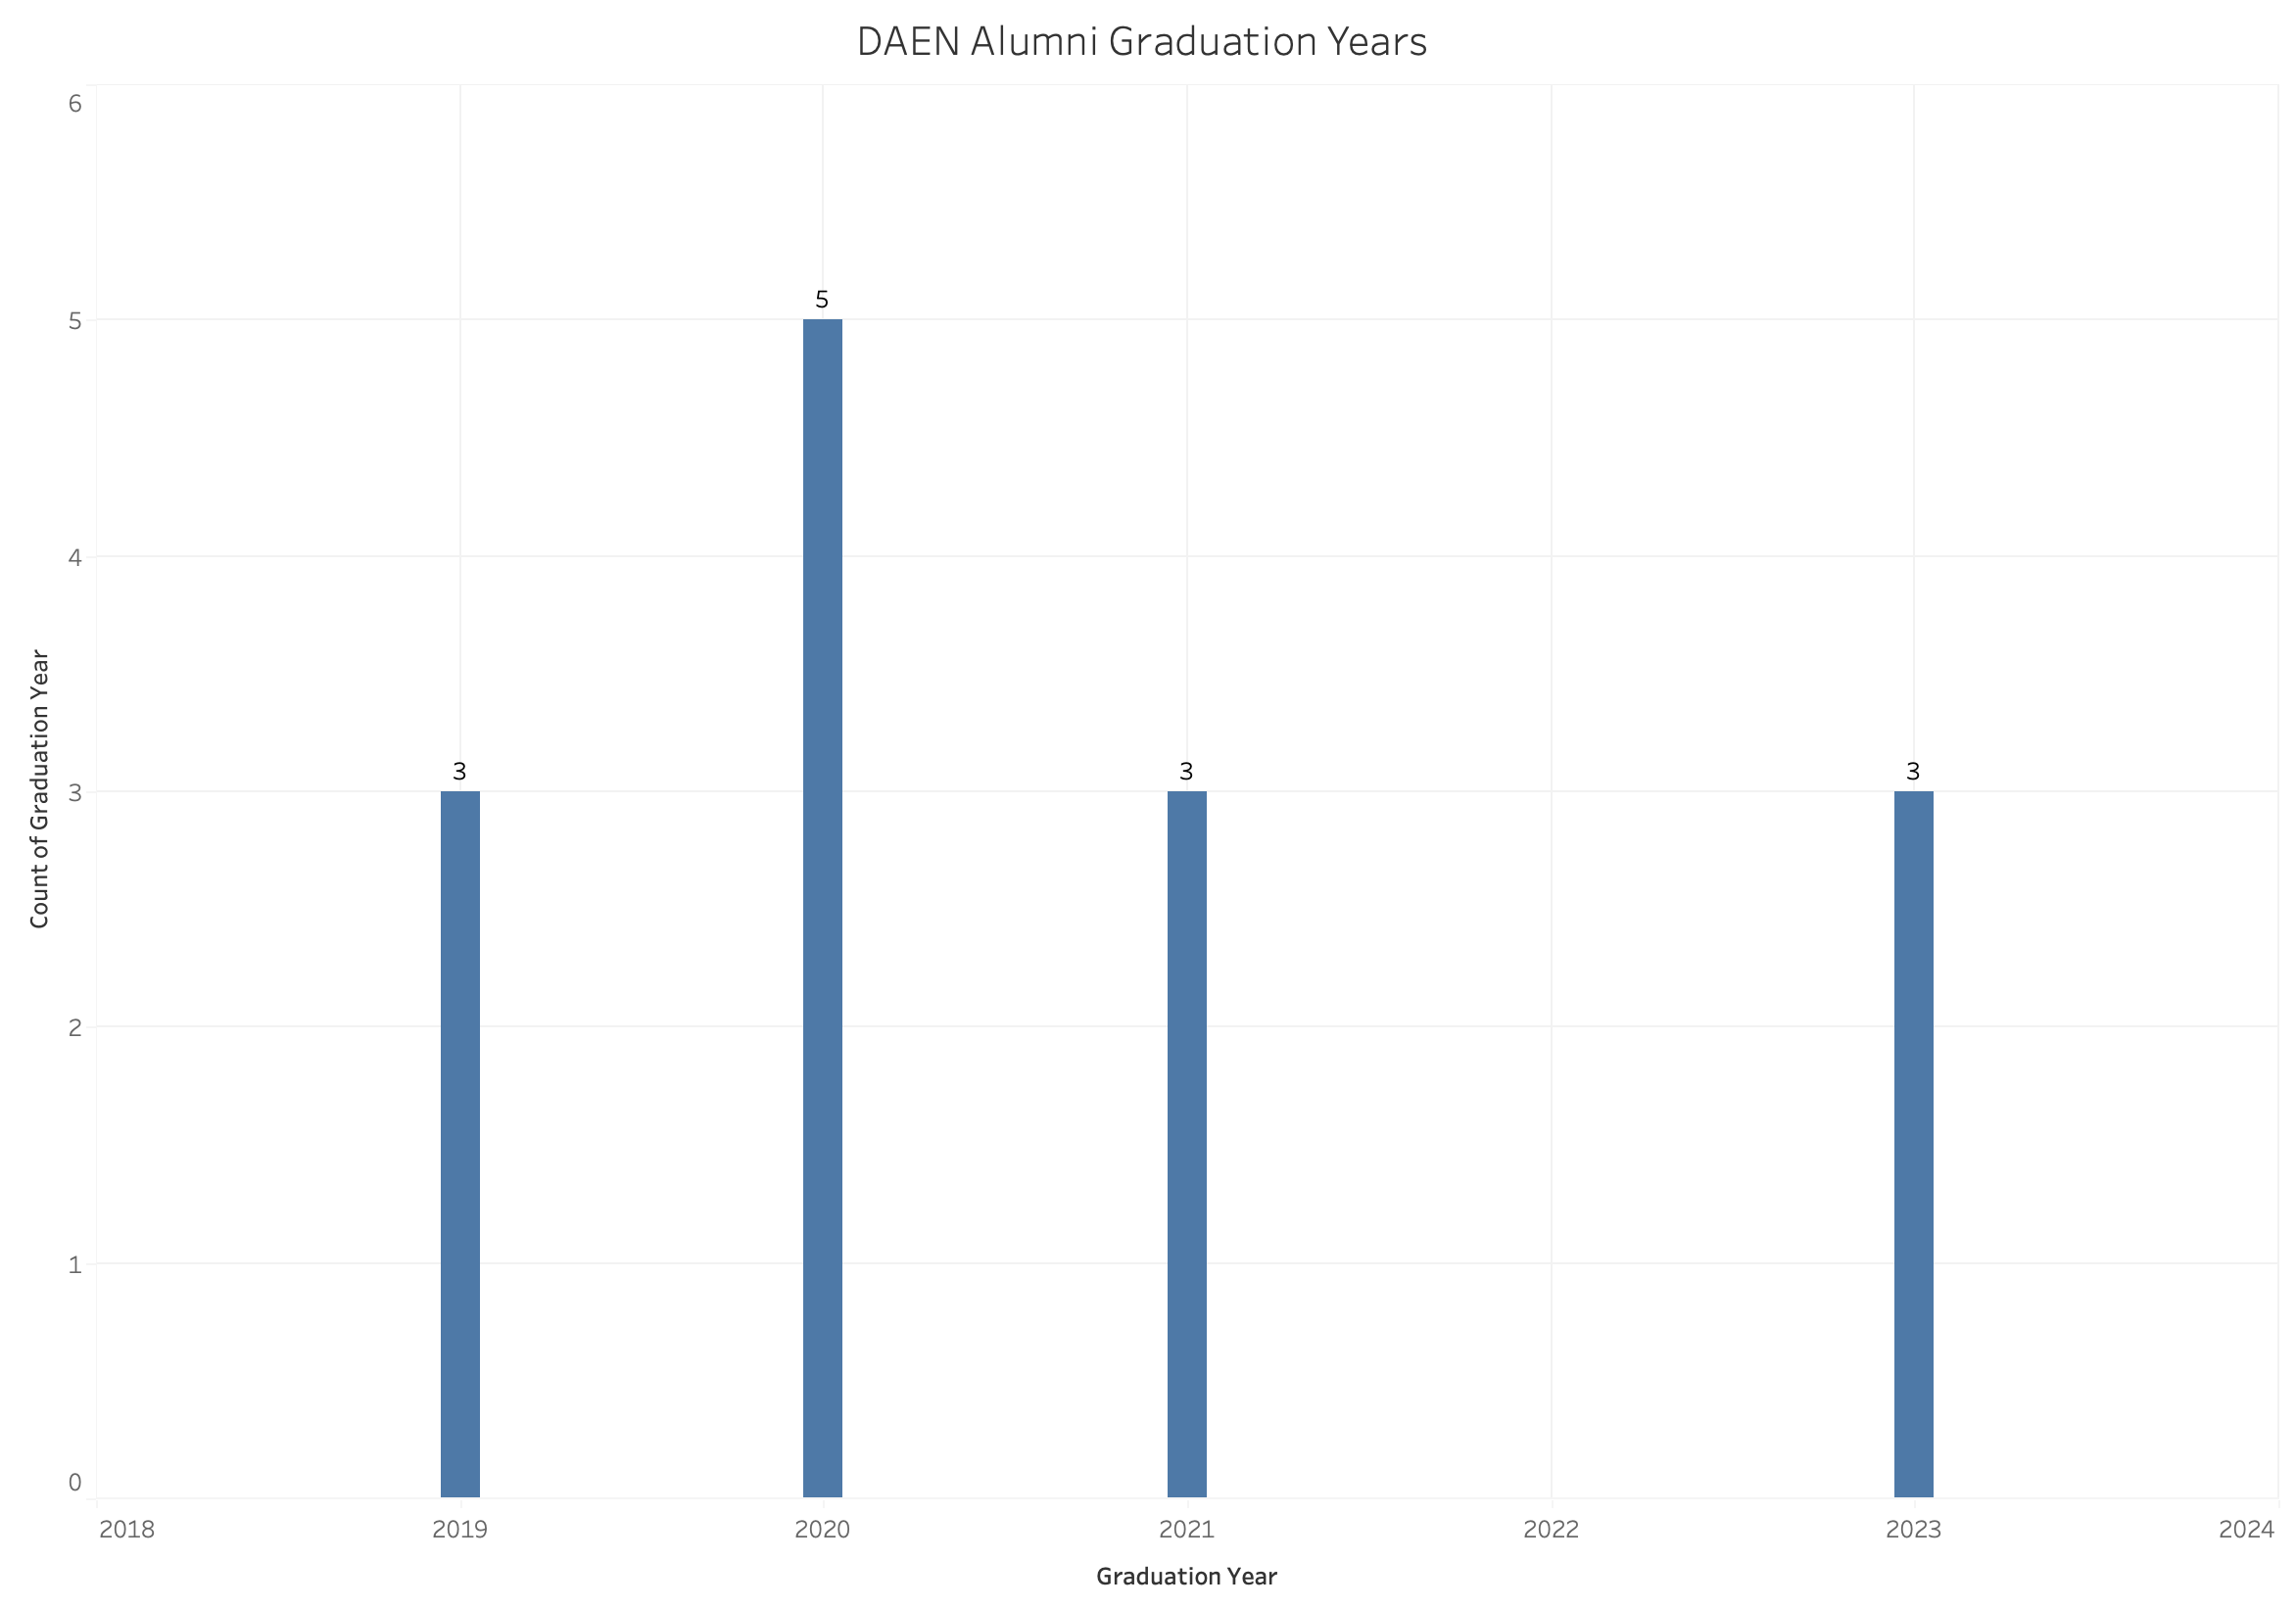
\includegraphics[width=0.9\textwidth]{visualizations/graduation-year.png}
    \caption{DAEN Alumni Graduation Year Distribution}
    \label{fig:graudation-year}
\end{figure}
\begin{figure}[H]
    \centering
    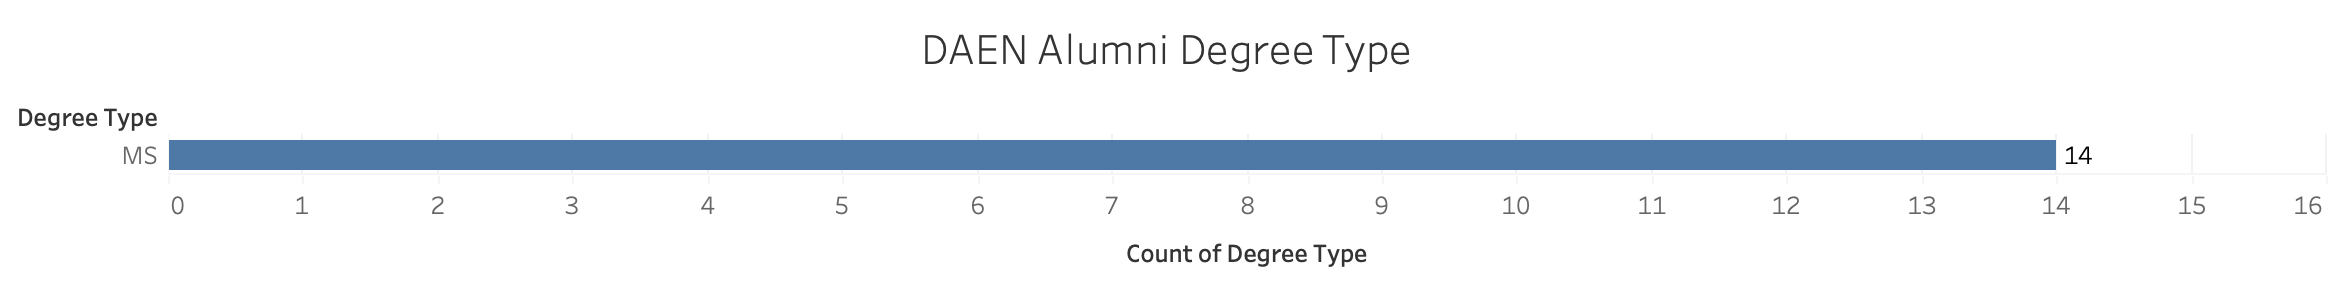
\includegraphics[width=0.9\textwidth]{visualizations/degree-type.png}
    \caption{DAEN Alumni Degree Type Distribution}
    \label{fig:degree-type}
\end{figure}

\begin{figure}[H]
    \centering
    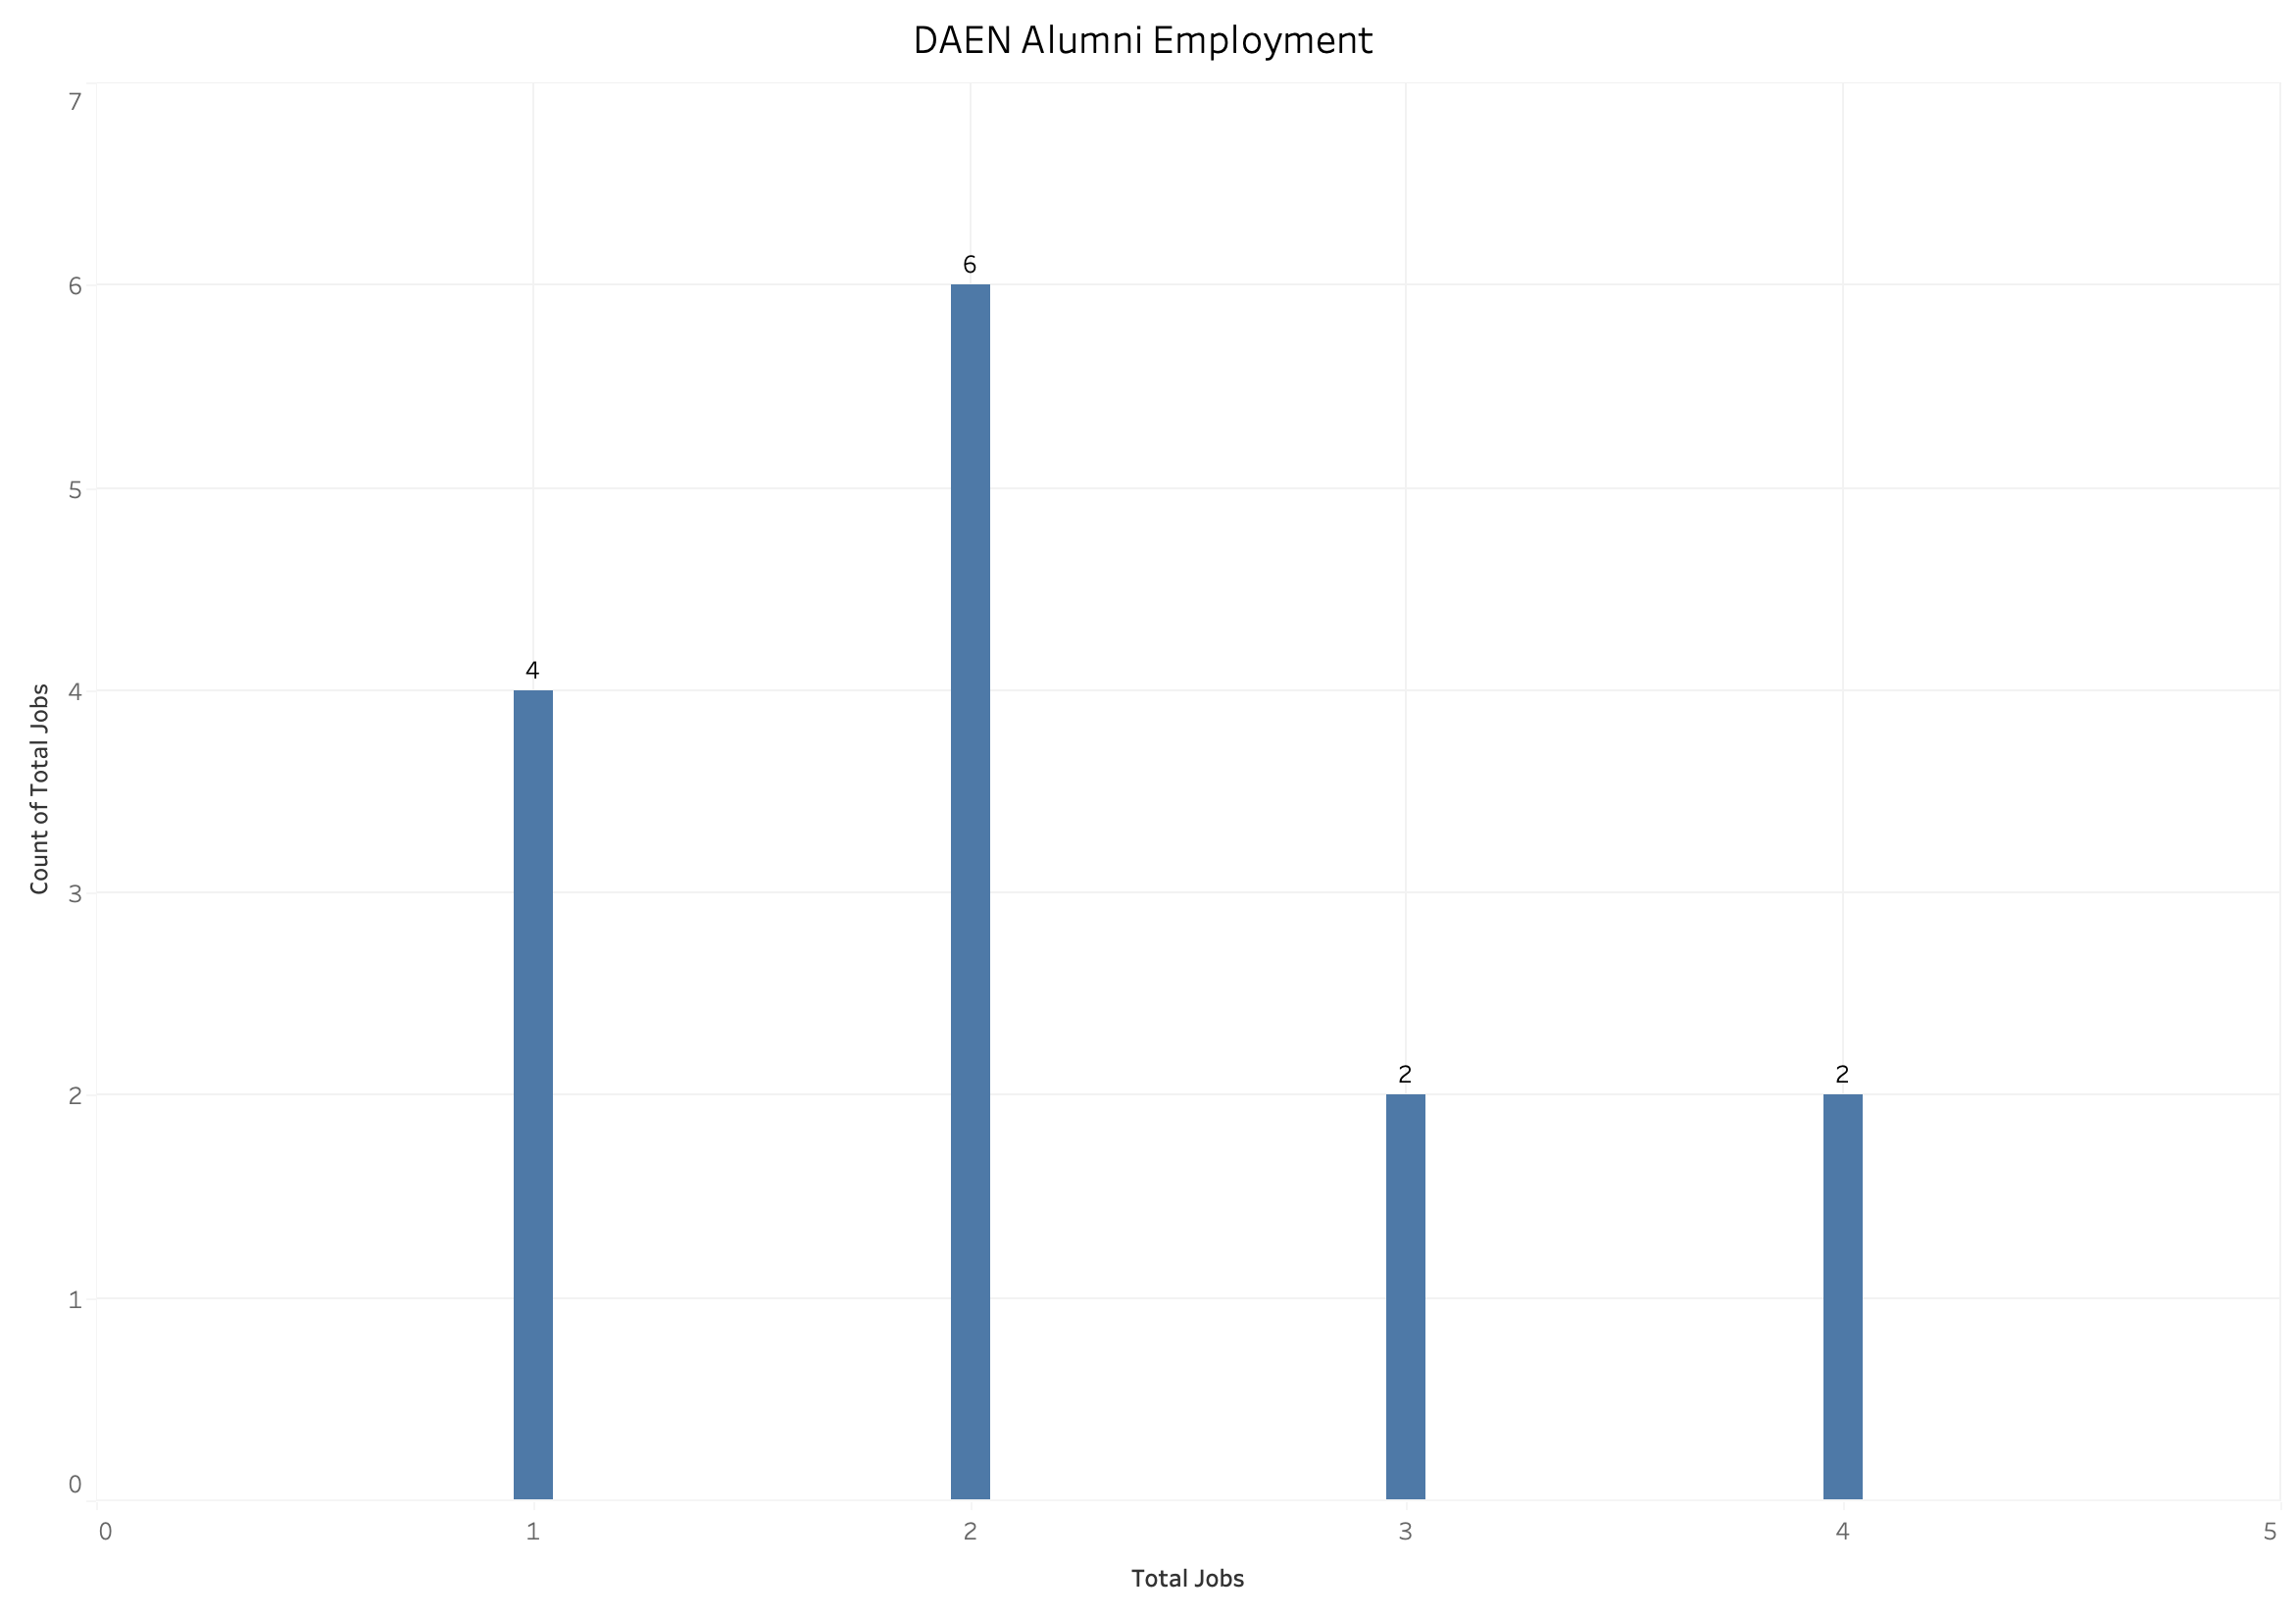
\includegraphics[width=0.9\textwidth]{visualizations/total-jobs.png}
    \caption{Total Jobs Held by DAEN Alumni}
    \label{fig:total-jobs}
\end{figure}

\begin{figure}[H]
    \centering
    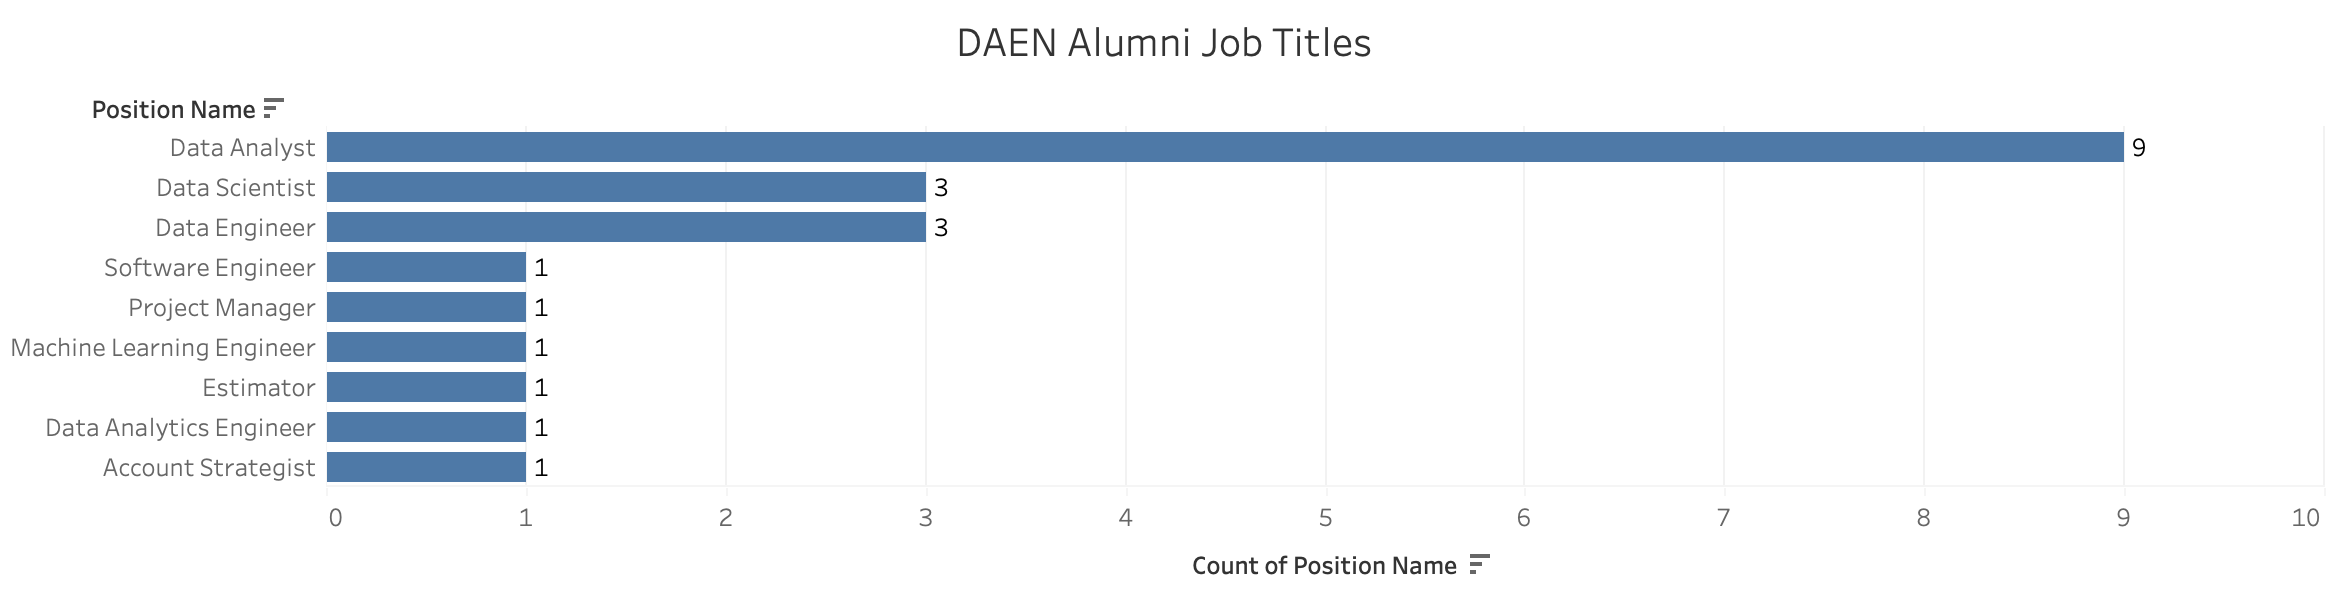
\includegraphics[width=0.9\textwidth]{visualizations/job-titles.png}
    \caption{Job Titles of DAEN Alumni}
    \label{fig:job-titles}
\end{figure}

\begin{figure}[H]
    \centering
    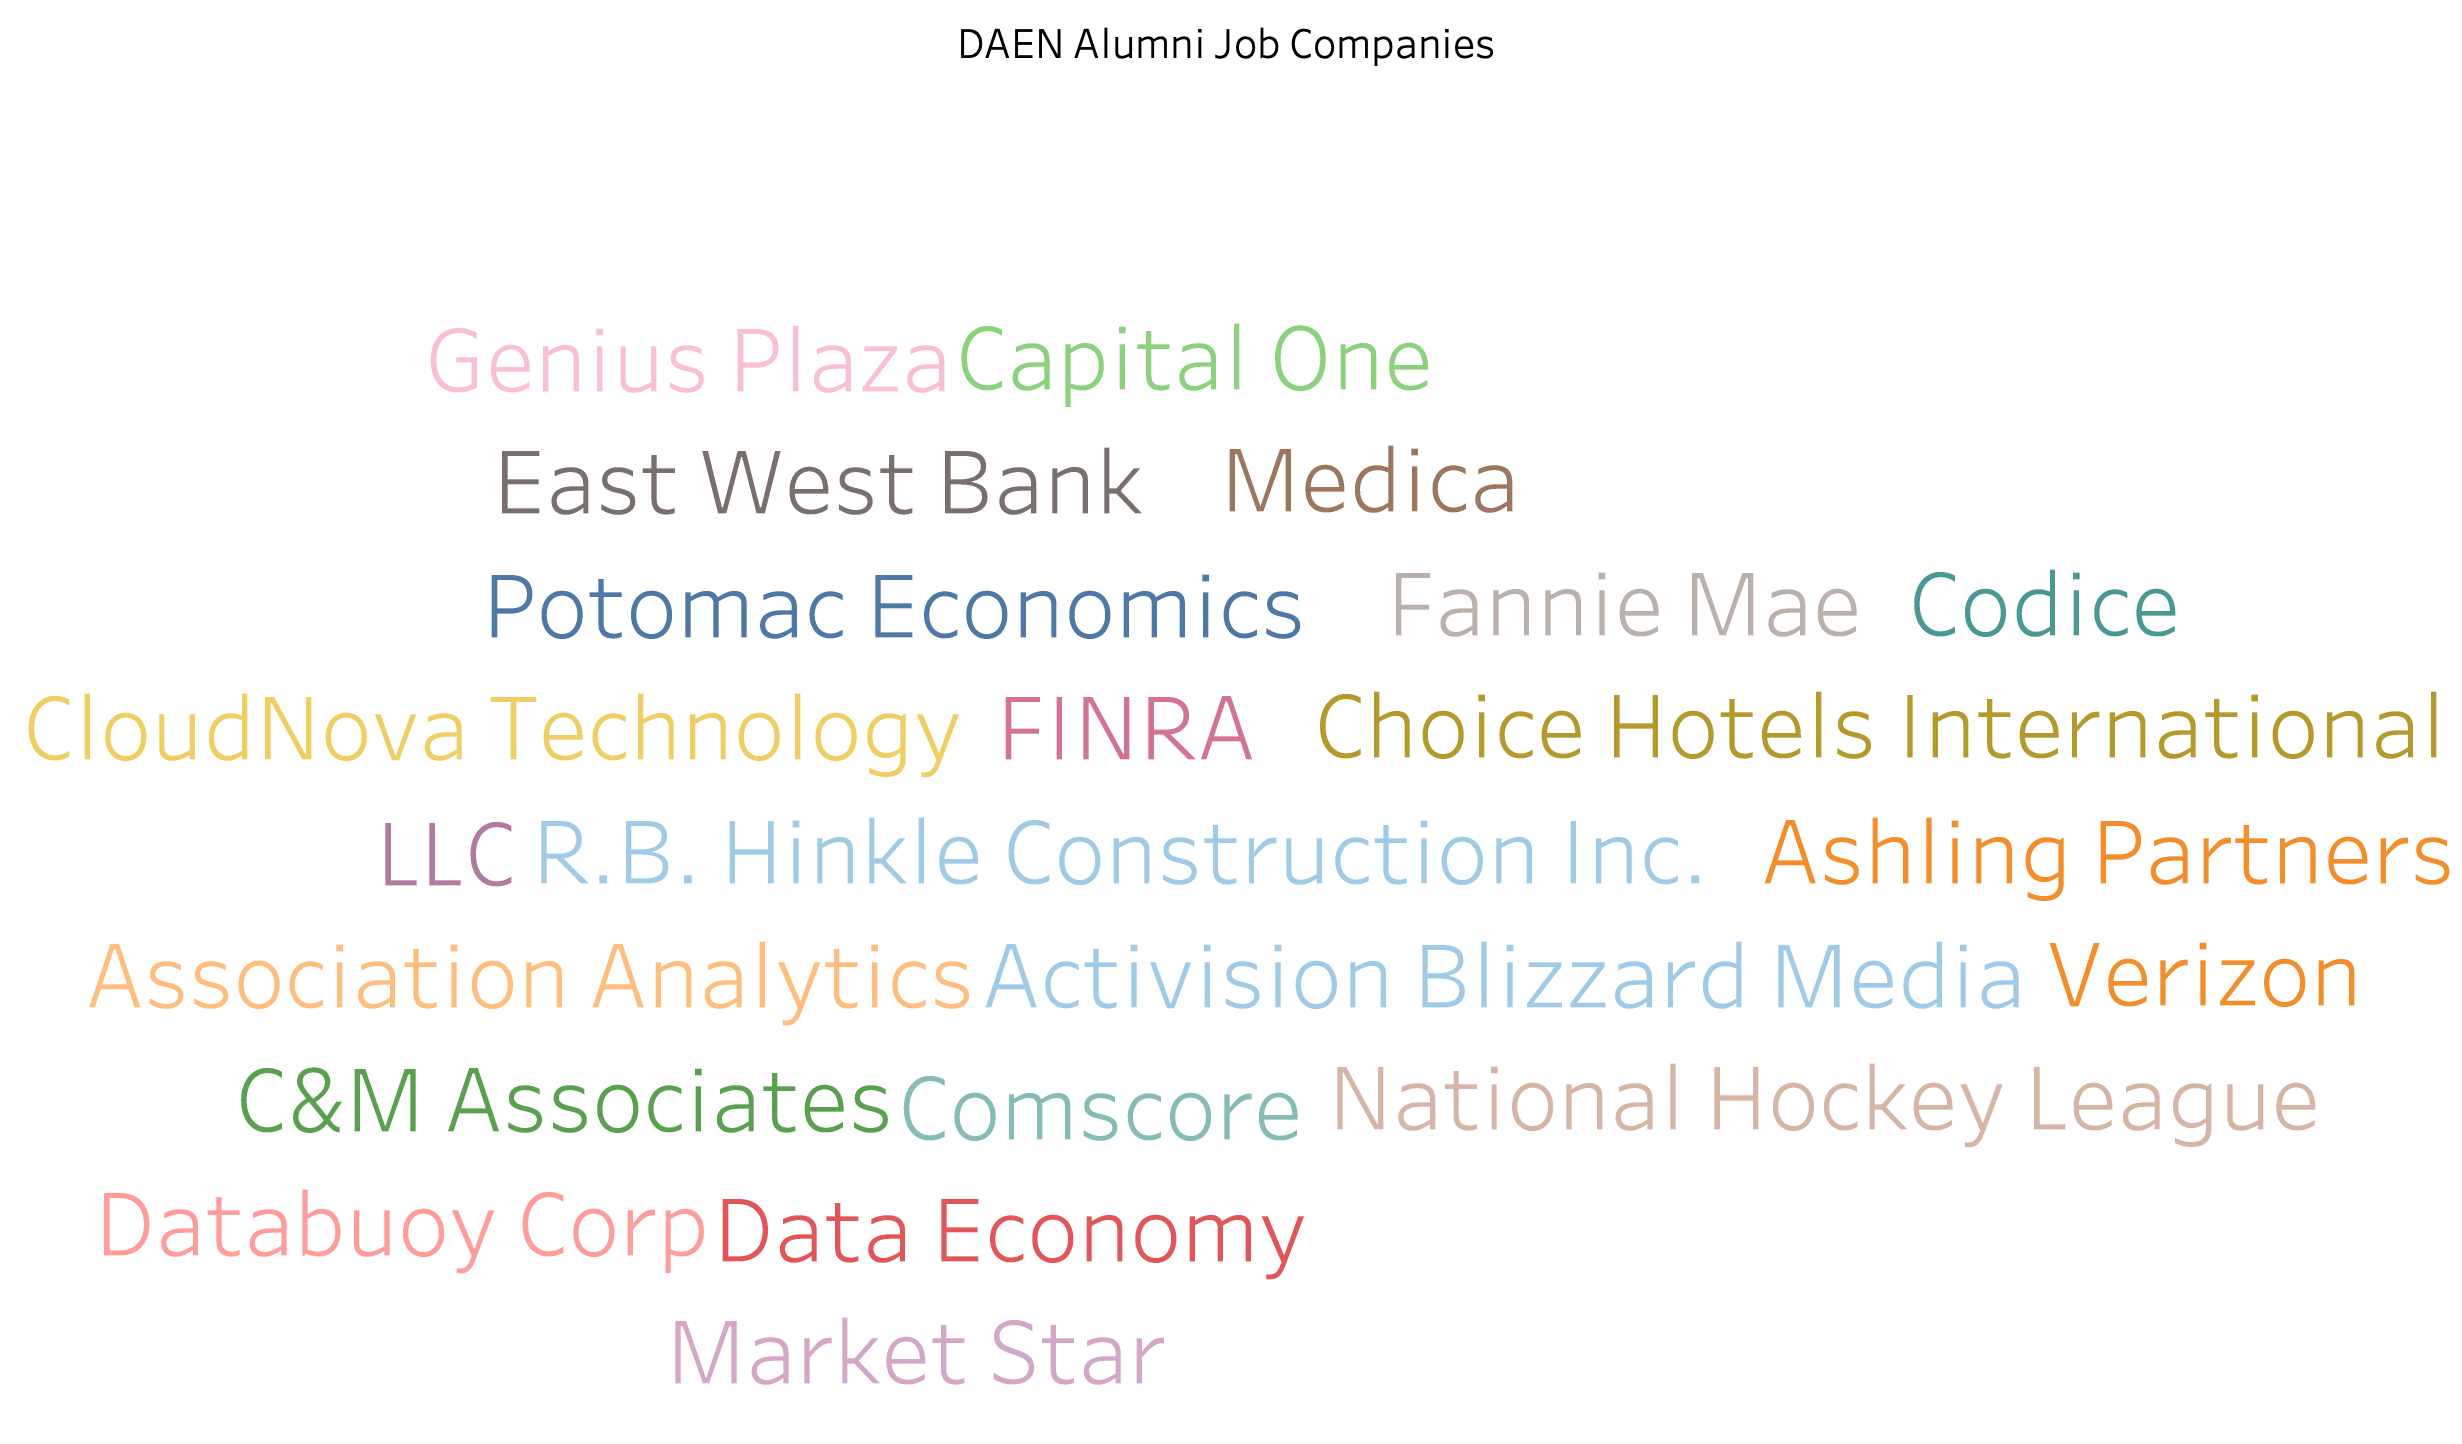
\includegraphics[width=0.9\textwidth]{visualizations/job-companies.png}
    \caption{Companies Employing DAEN Alumni}
    \label{fig:job-companies}
\end{figure}

\begin{figure}[H]
    \centering
    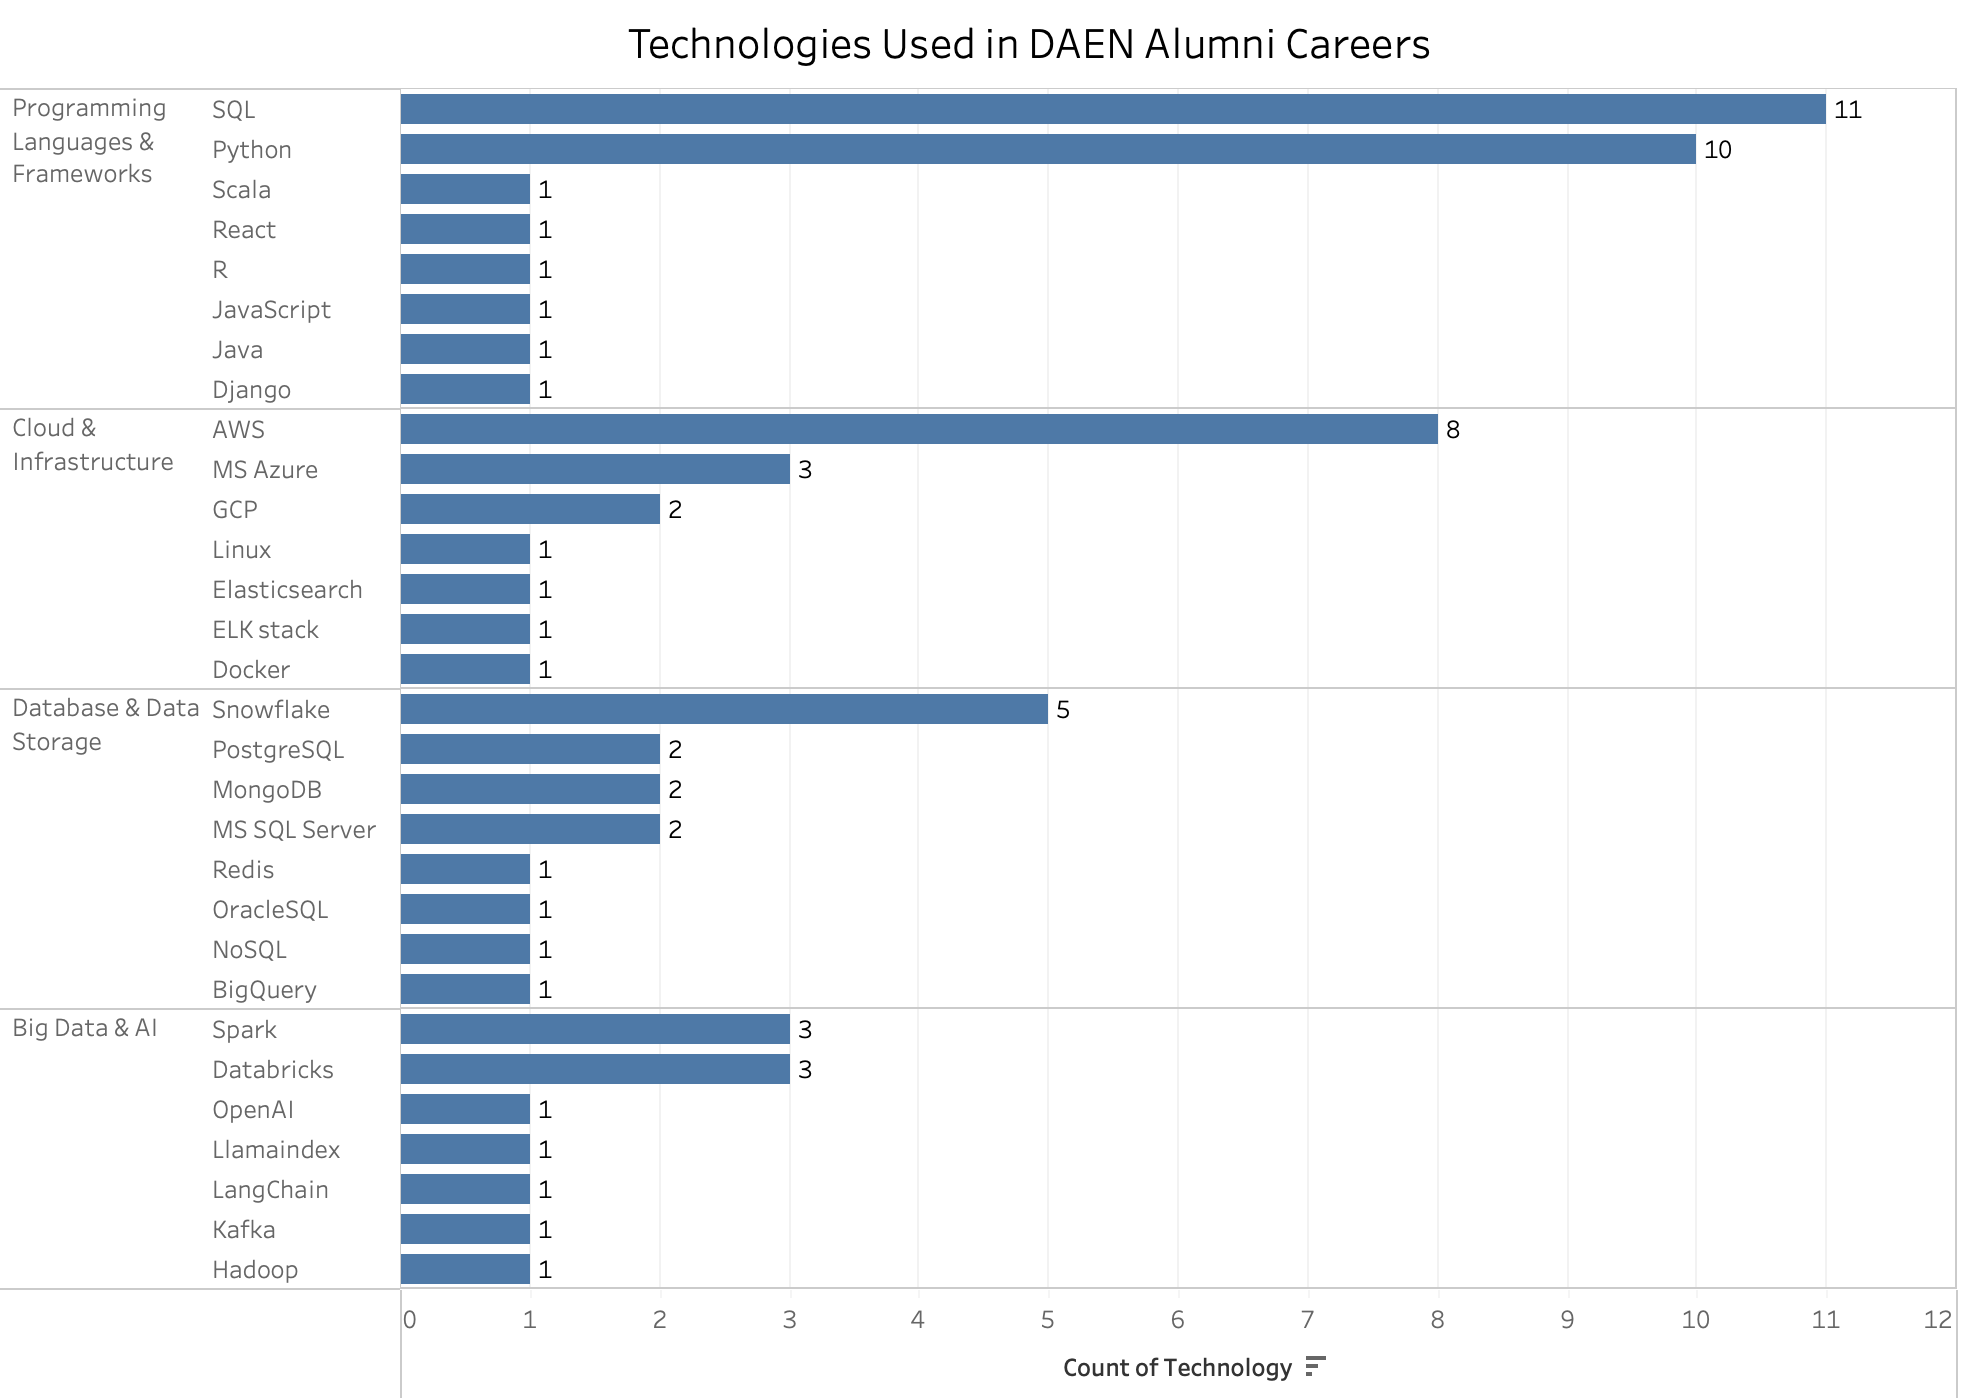
\includegraphics[width=0.9\textwidth]{visualizations/career-technologies.png}
    \caption{Technologies Used in DAEN Alumni Careers}
    \label{fig:career-technologies}
\end{figure}

\begin{figure}[H]
    \centering
    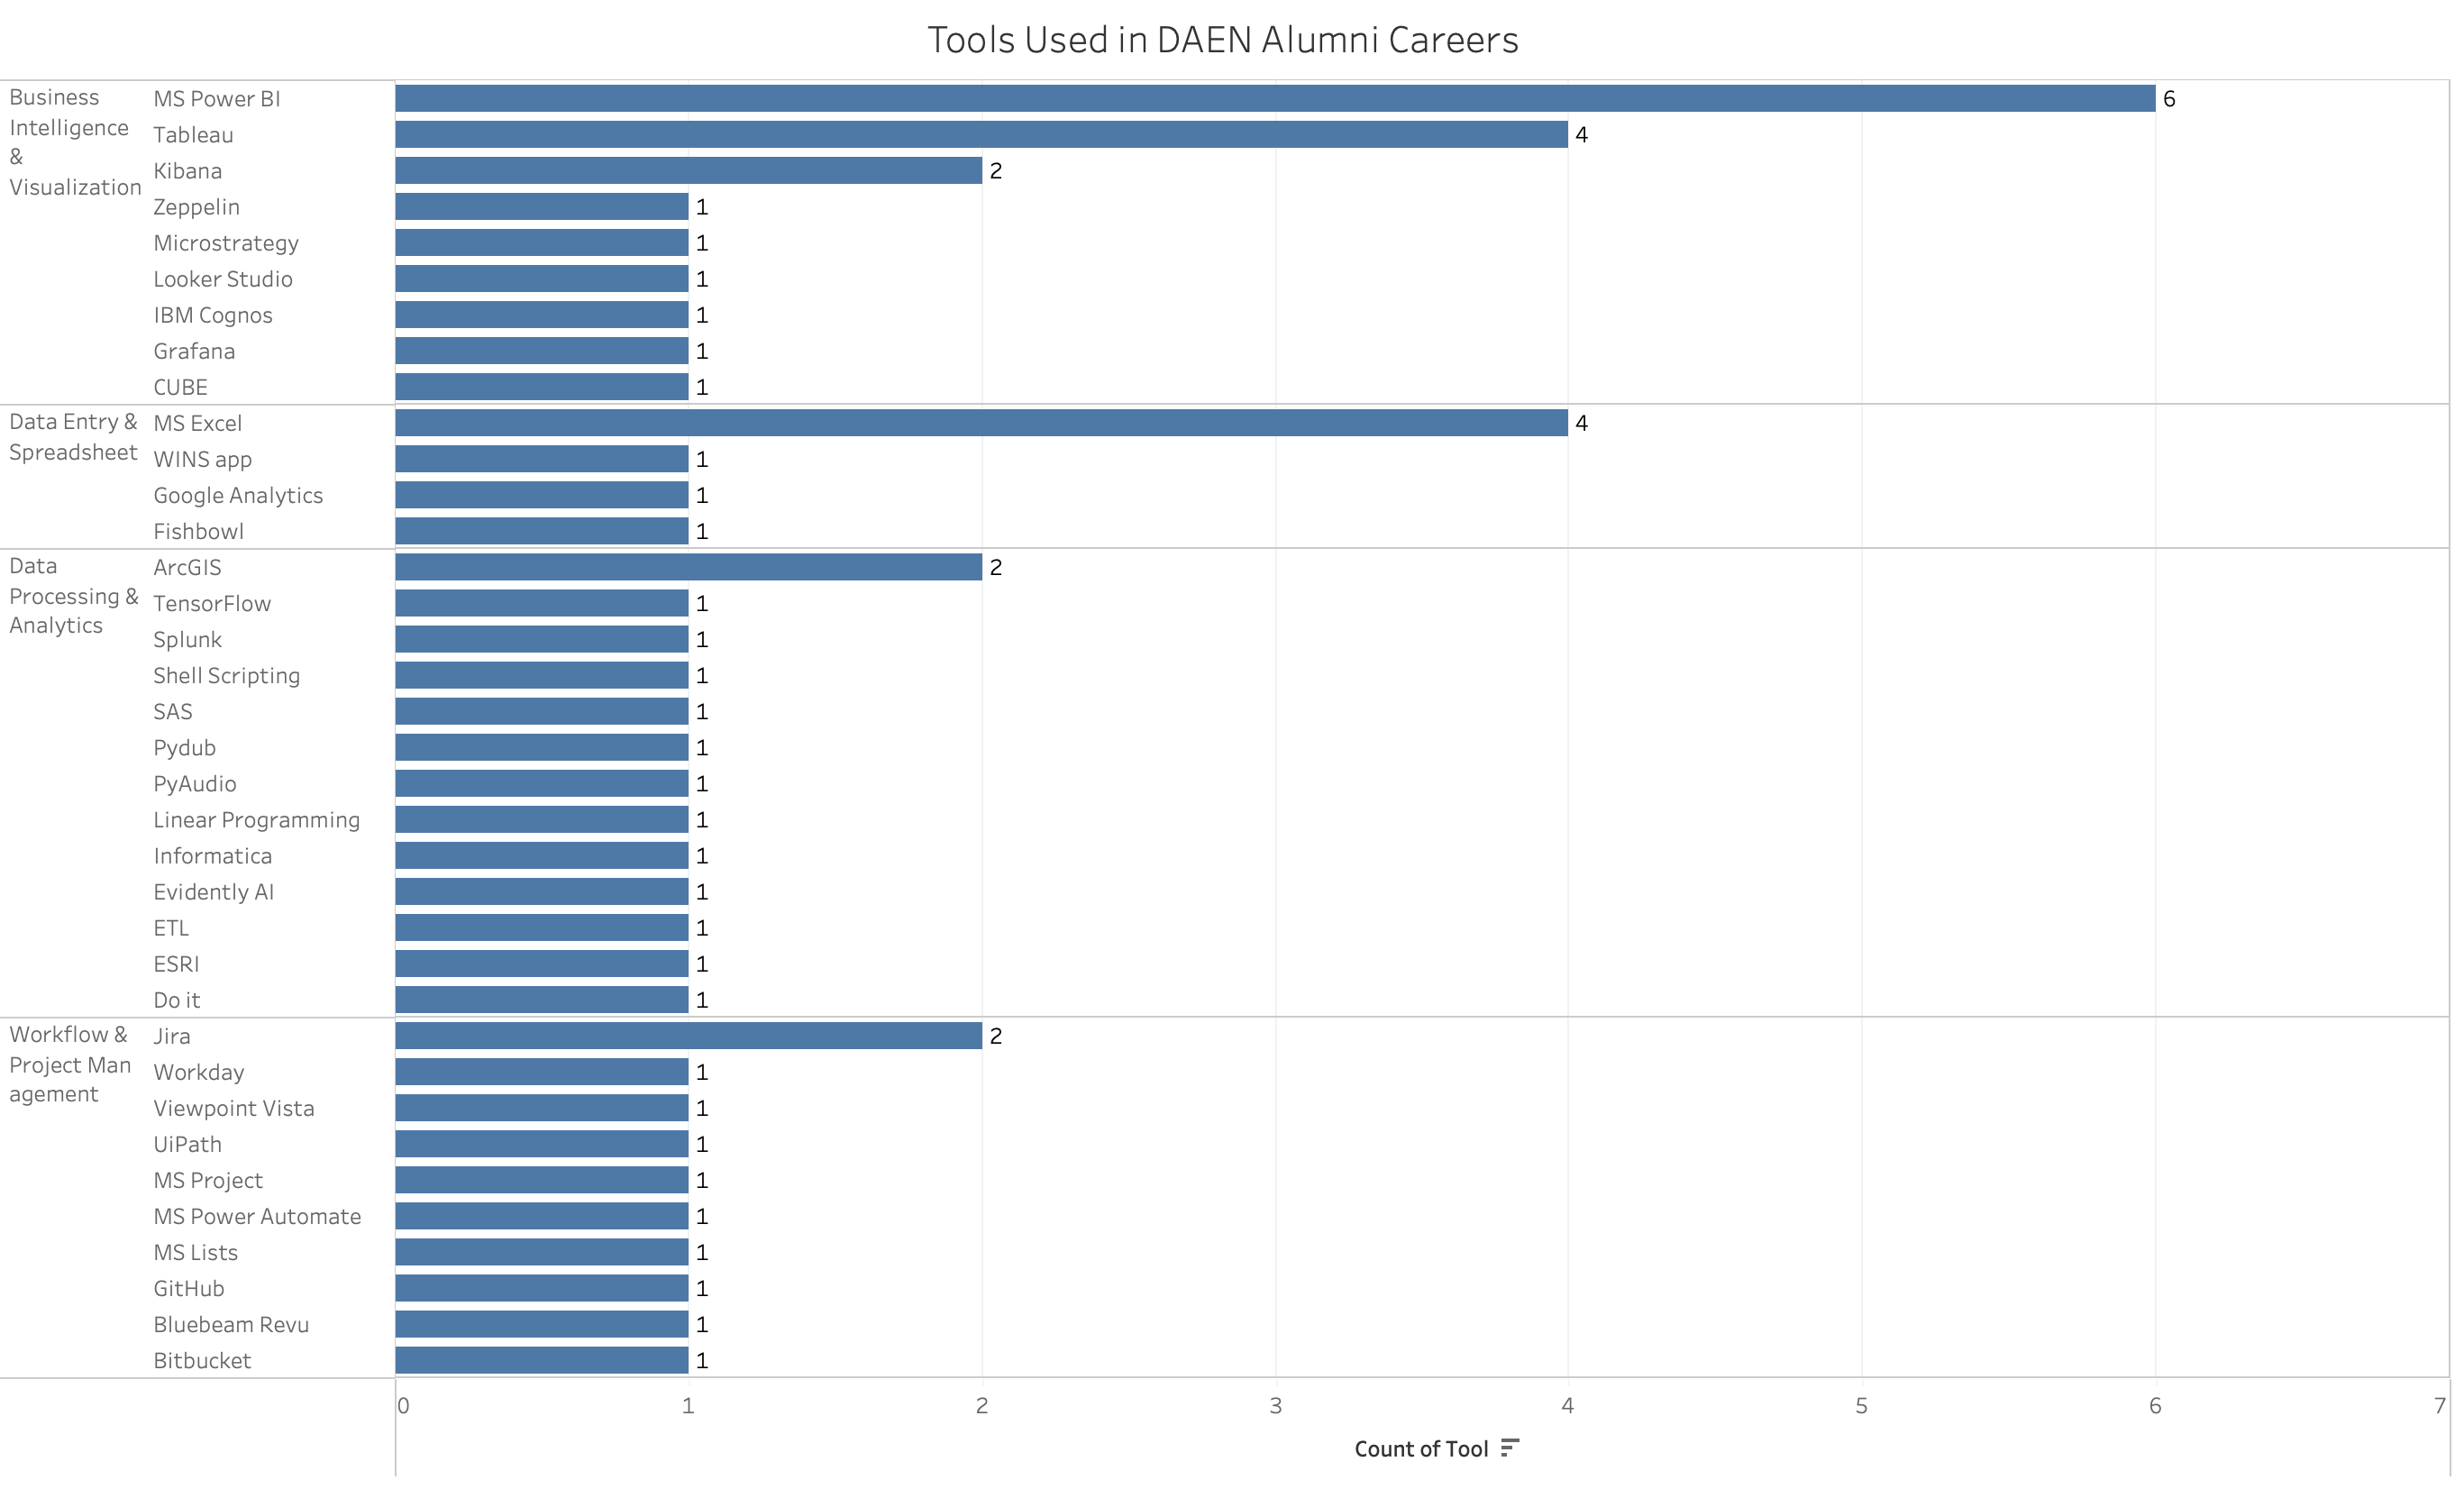
\includegraphics[width=0.9\textwidth]{visualizations/career-tools.png}
    \caption{Tools Used in DAEN Alumni Careers}
    \label{fig:career-tools}
\end{figure}

\begin{figure}[H]
    \centering
    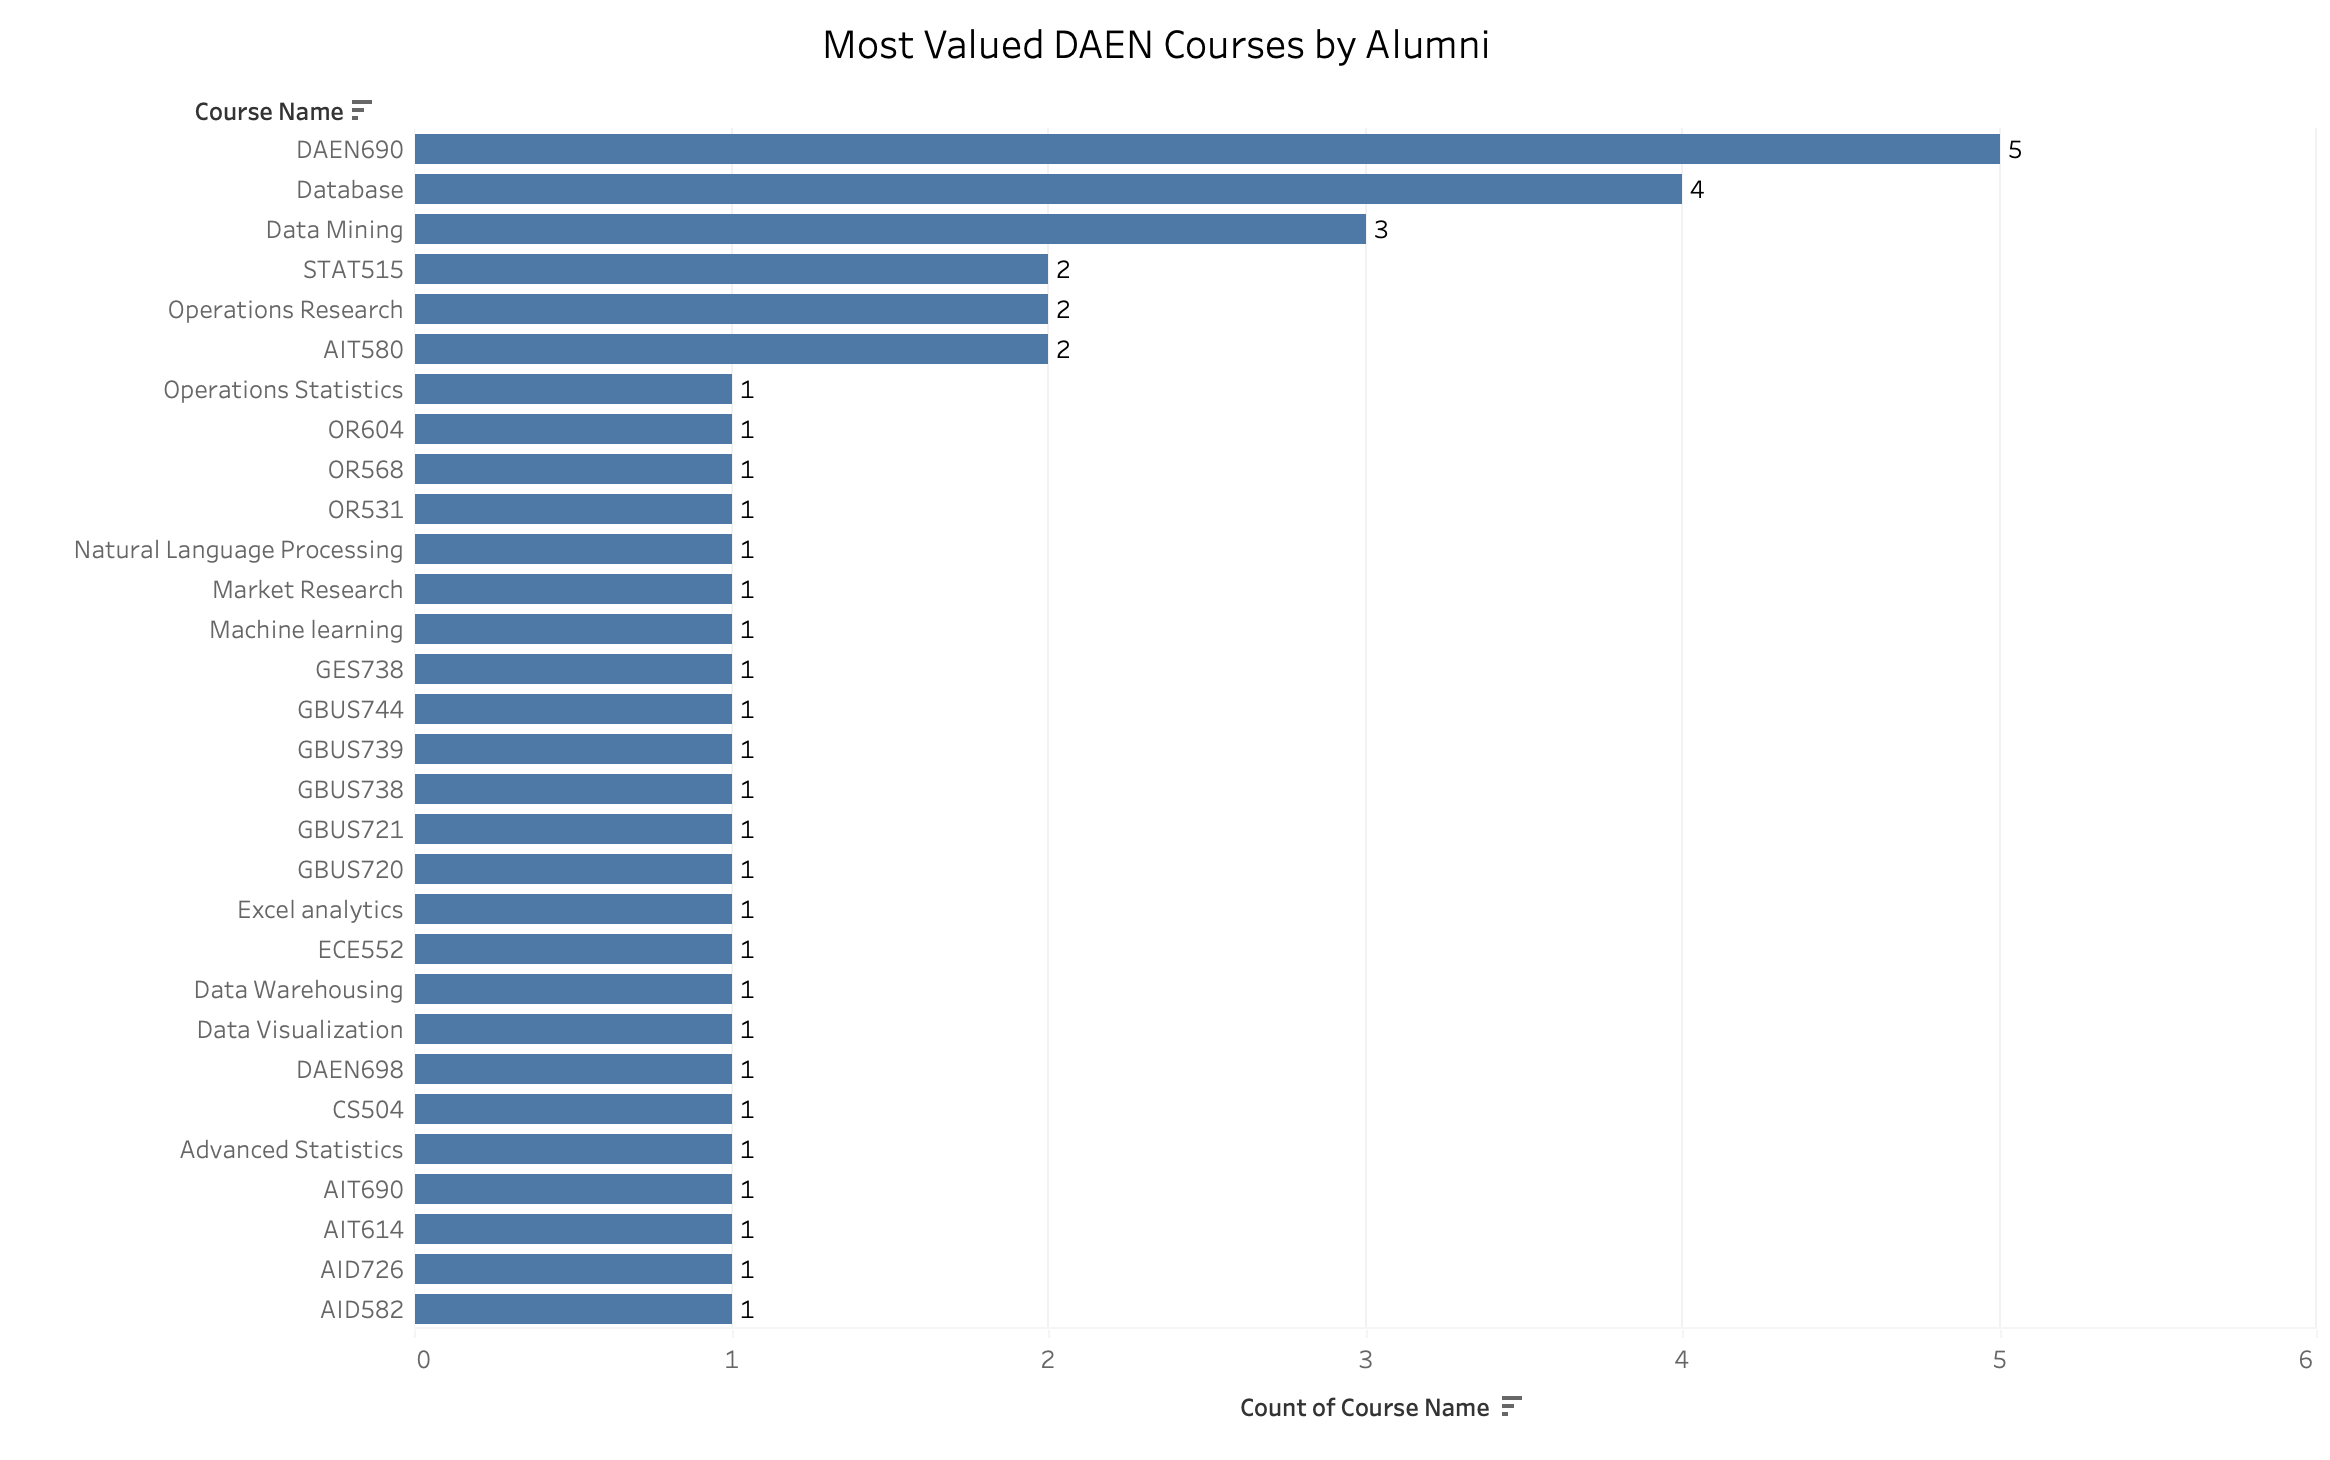
\includegraphics[width=0.9\textwidth]{visualizations/daen-courses.png}
    \caption{Valuable Program Courses}
    \label{fig:daen-courses}
\end{figure}

\begin{figure}[H]
    \centering
    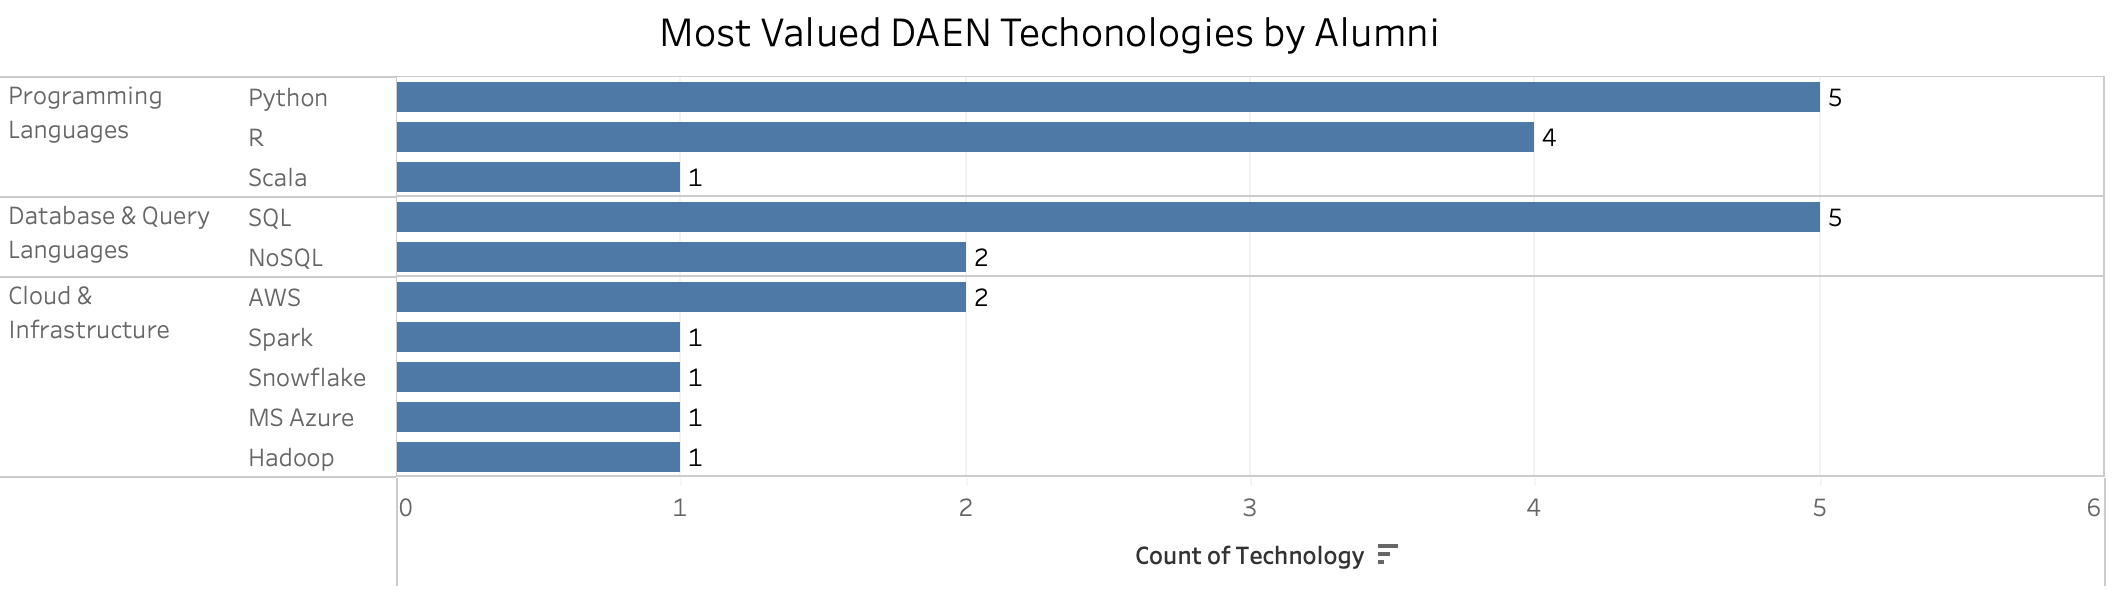
\includegraphics[width=0.9\textwidth]{visualizations/daen-technologies.png}
    \caption{Valuable Technologies Acquired in DAEN Program}
    \label{fig:daen-technologies}
\end{figure}

\begin{figure}[H]
    \centering
    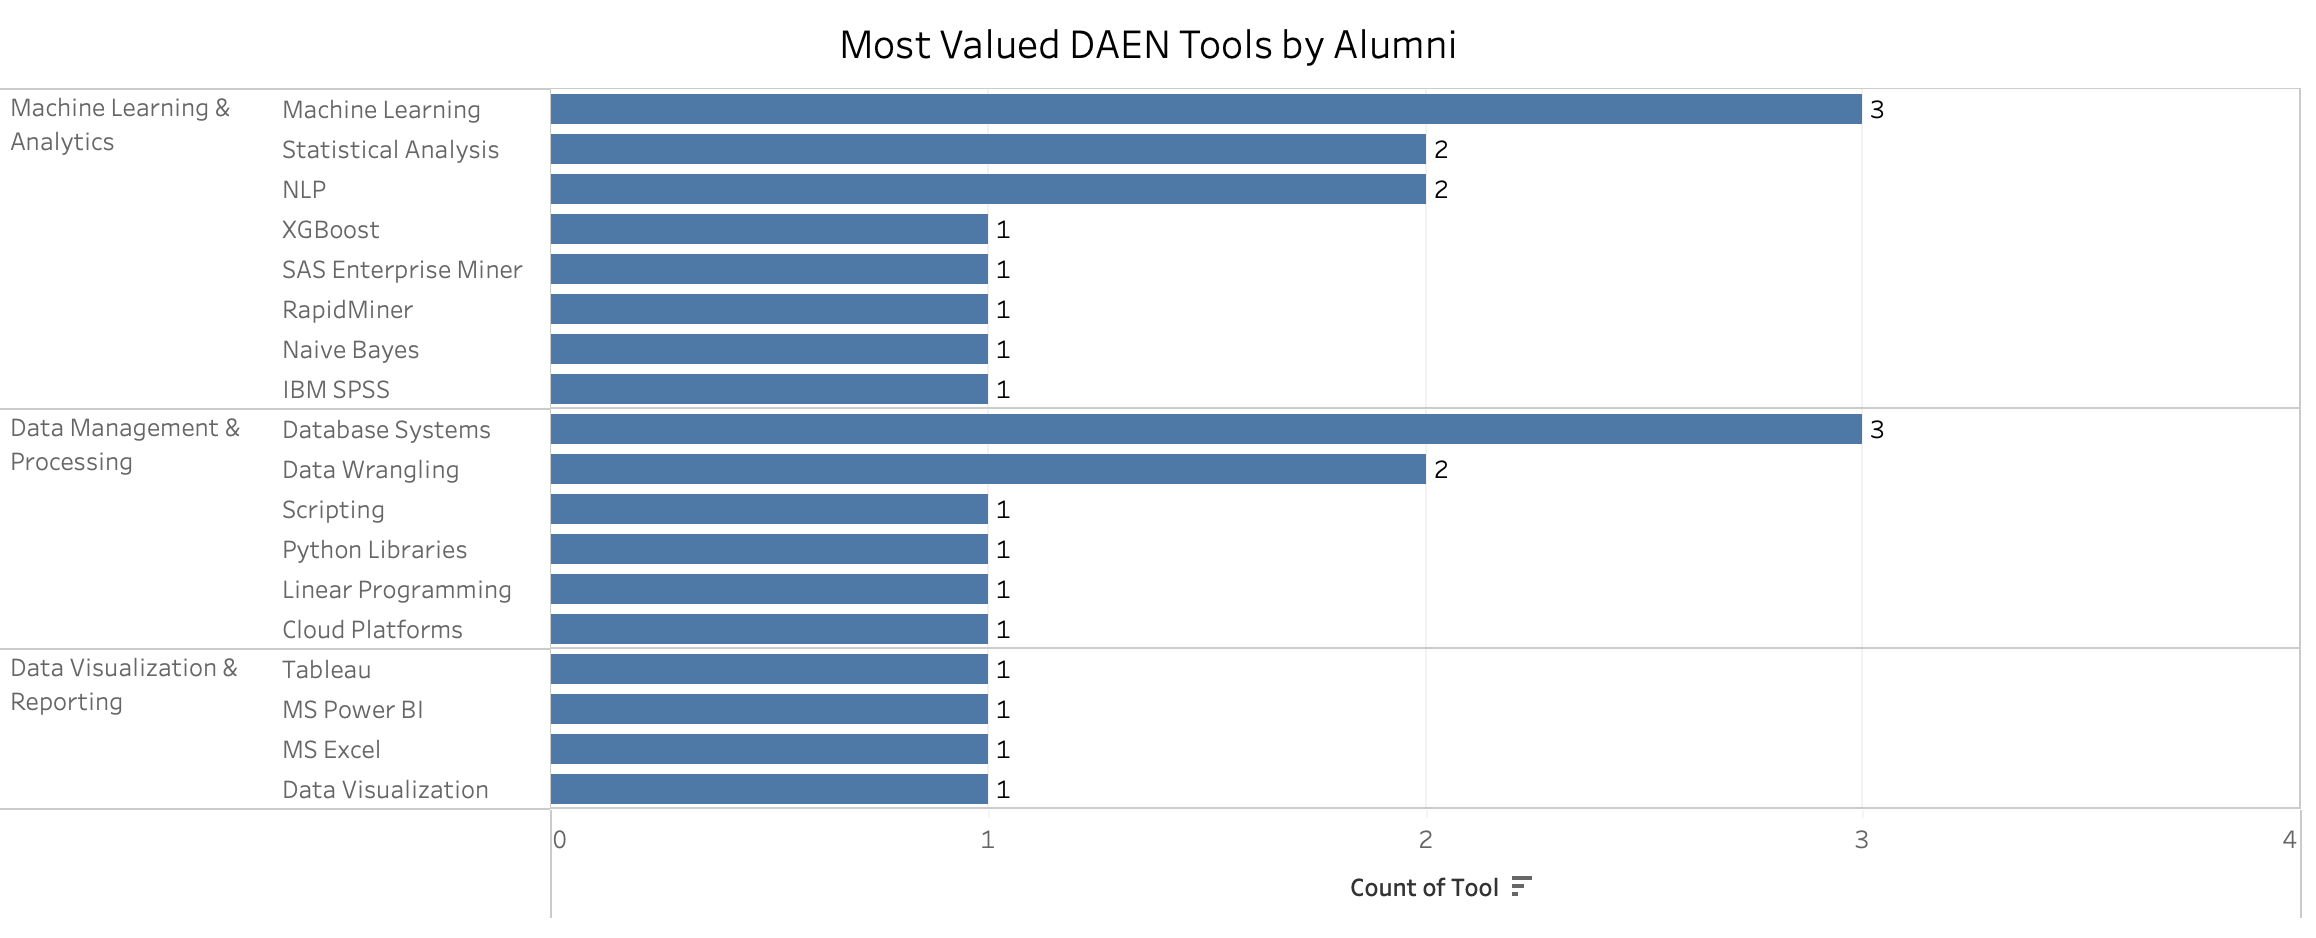
\includegraphics[width=0.9\textwidth]{visualizations/daen-tools.png}
    \caption{Valuable Tools Acquired in DAEN Program}
    \label{fig:daen-tools}
\end{figure}

\begin{figure}[H]
    \centering
    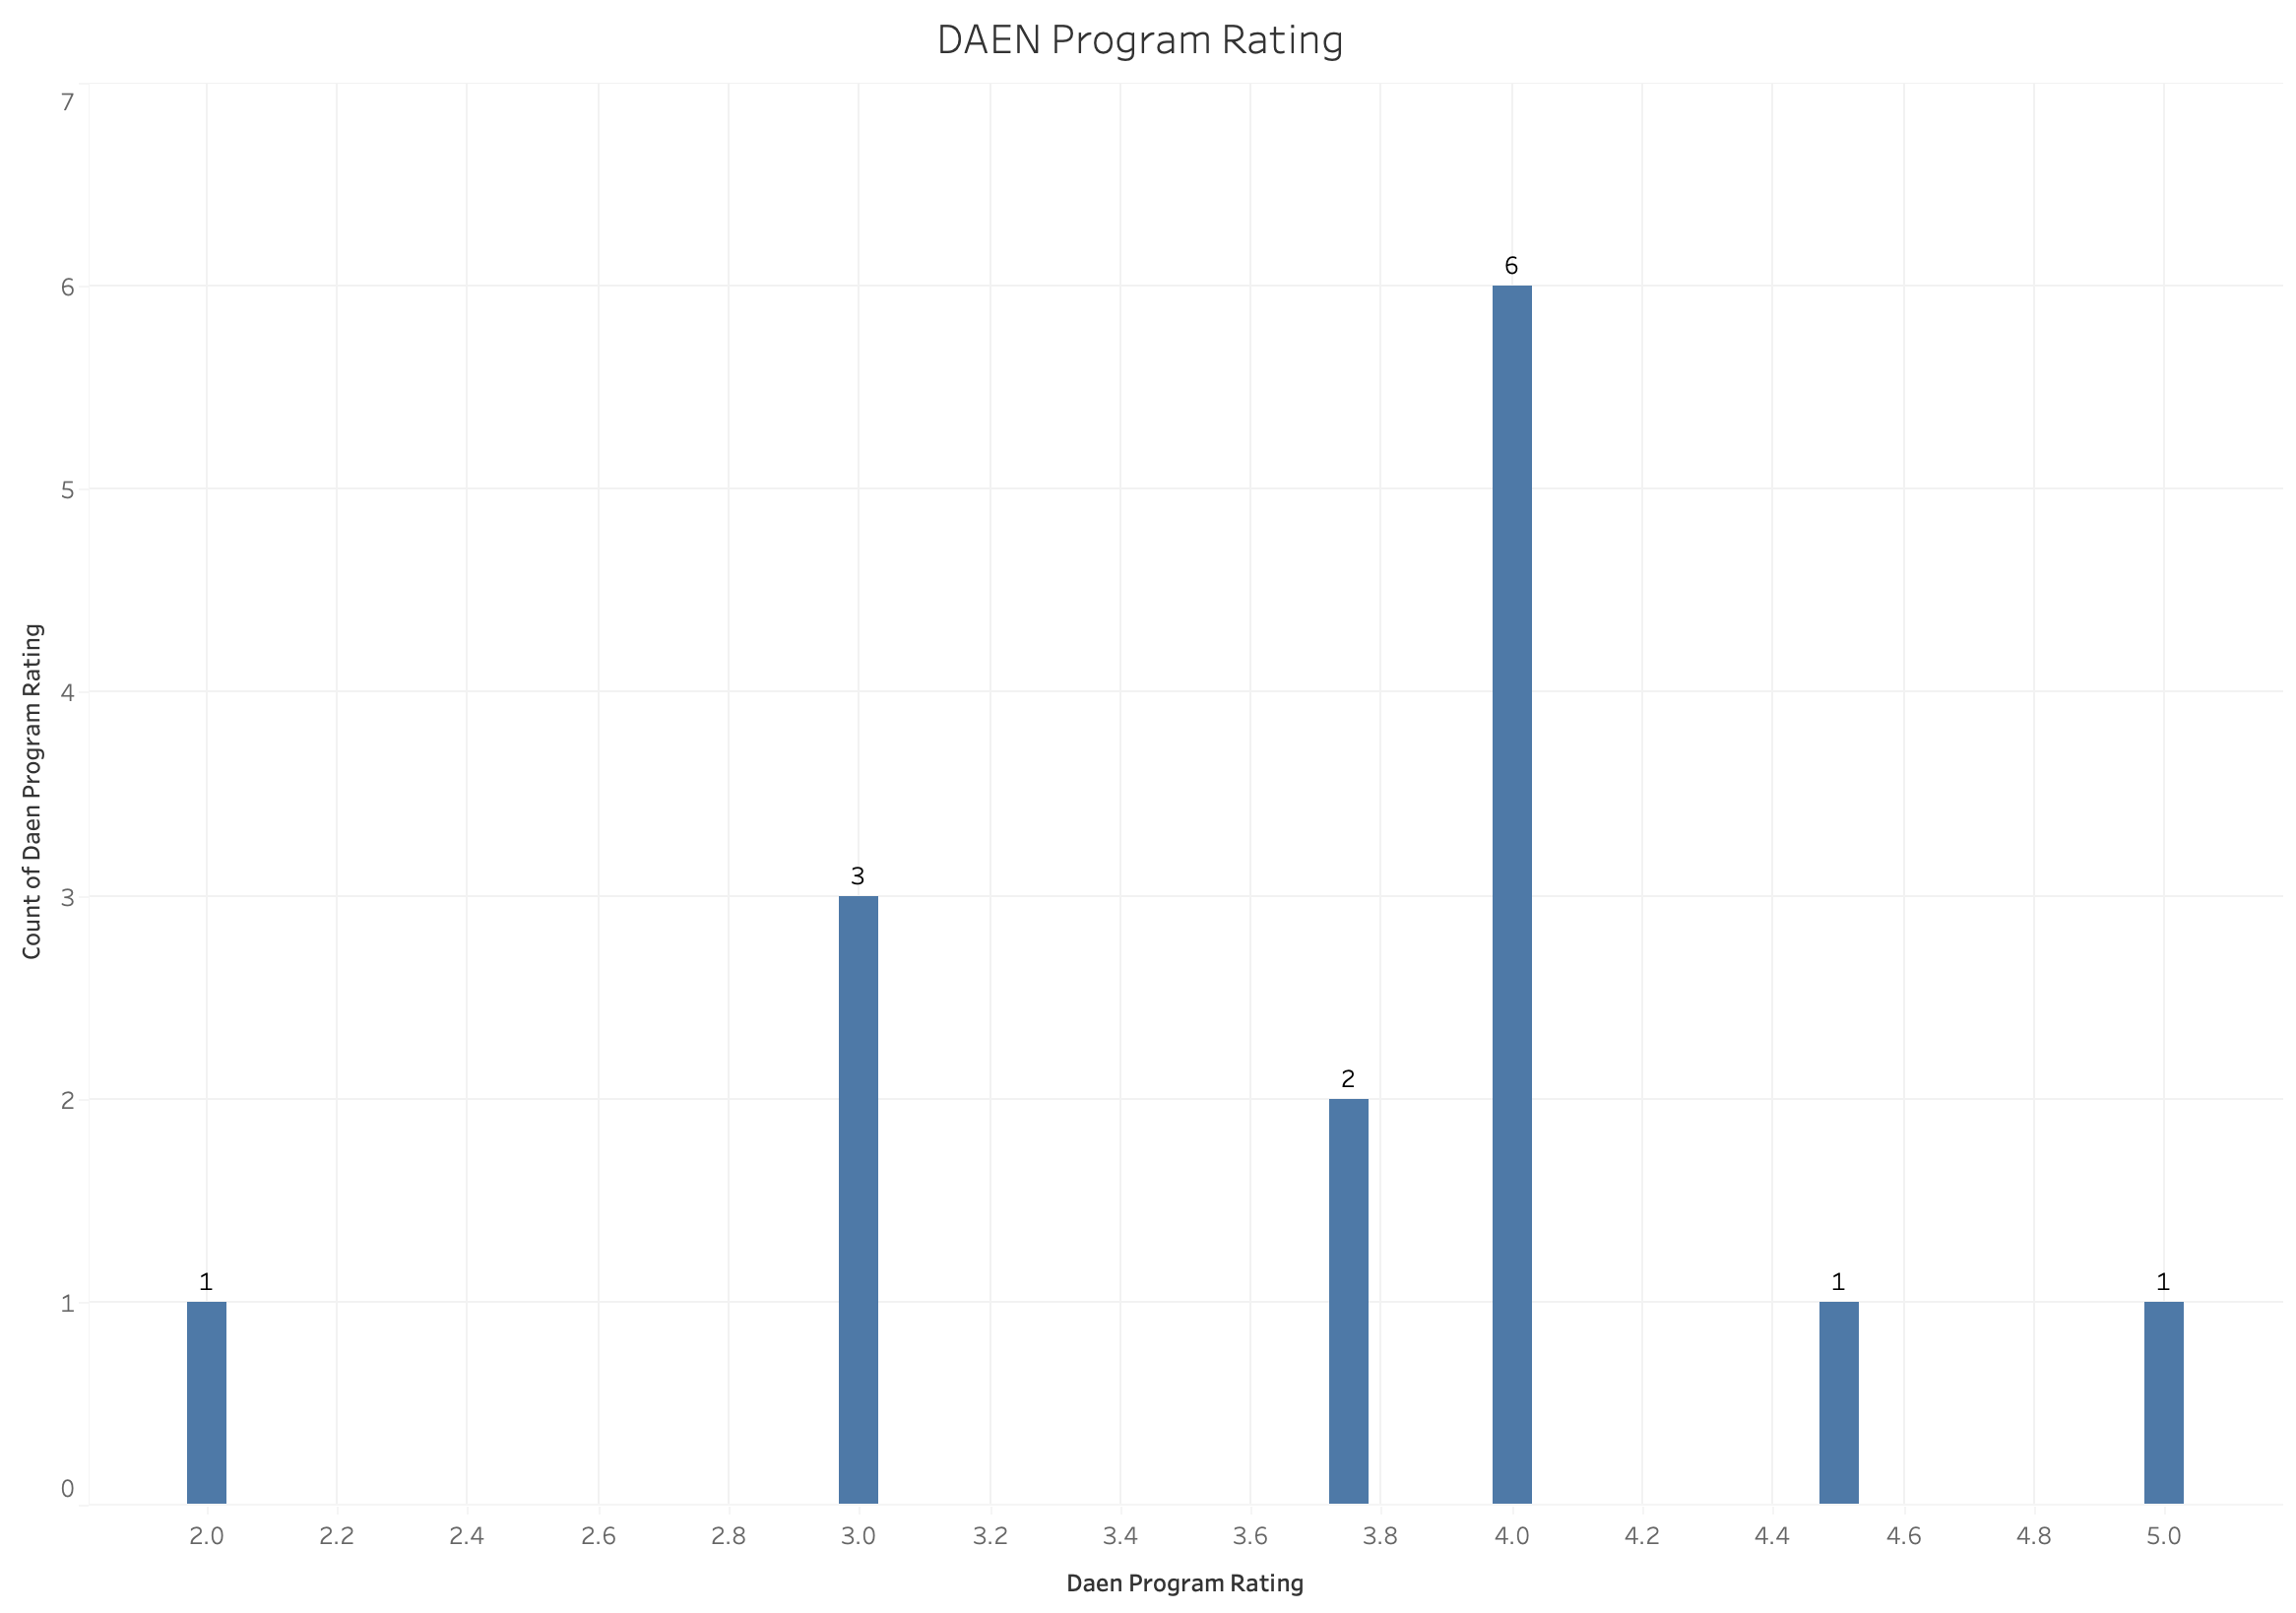
\includegraphics[width=0.9\textwidth]{visualizations/daen-rating.png}
    \caption{DAEN Alumni Program Ratings}
    \label{fig:daen-rating}
\end{figure}

\begin{figure}[H]
    \centering
    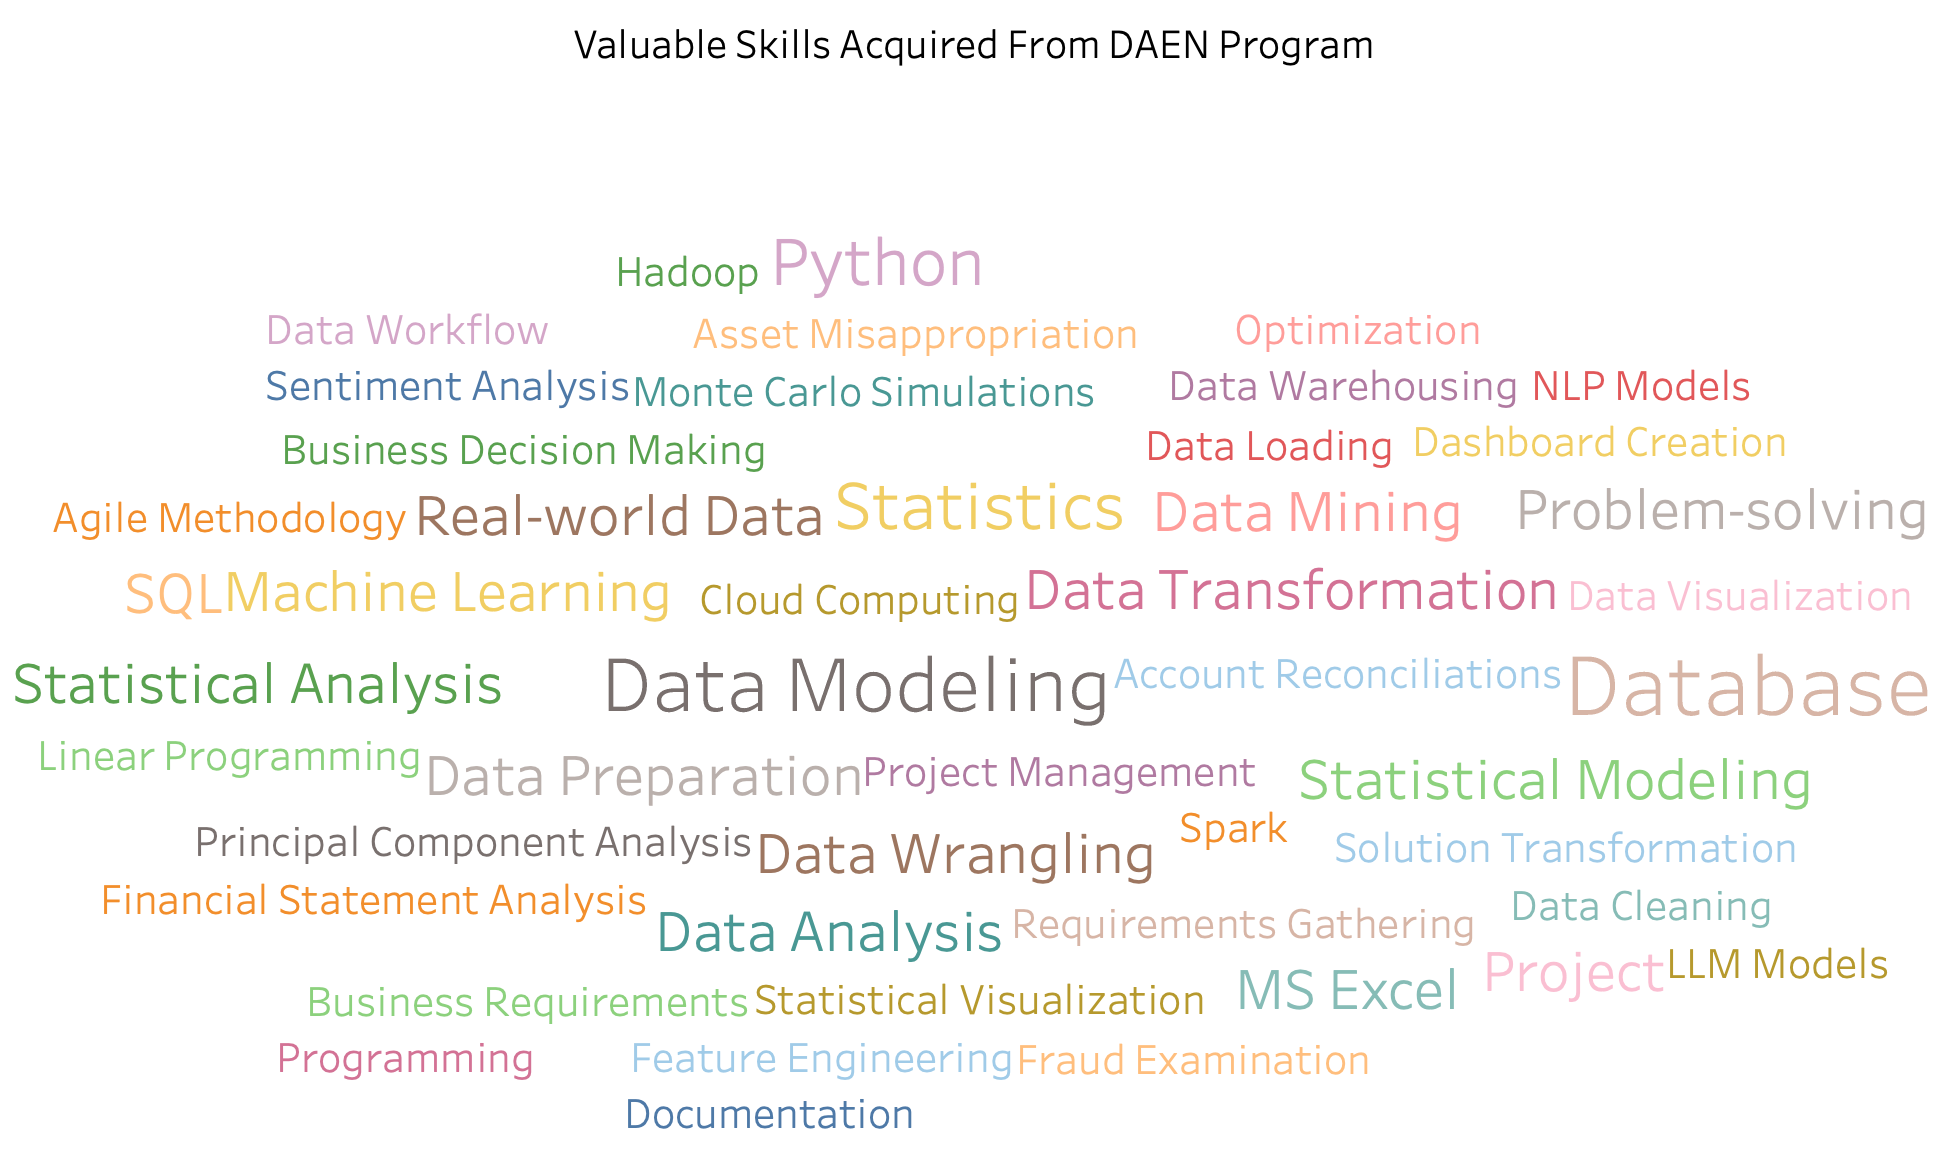
\includegraphics[width=0.9\textwidth]{visualizations/program-skills.png}
    \caption{Valuable Skills Acquired in DAEN Program}
    \label{fig:program-skills}
\end{figure}

\begin{figure}[H]
    \centering
    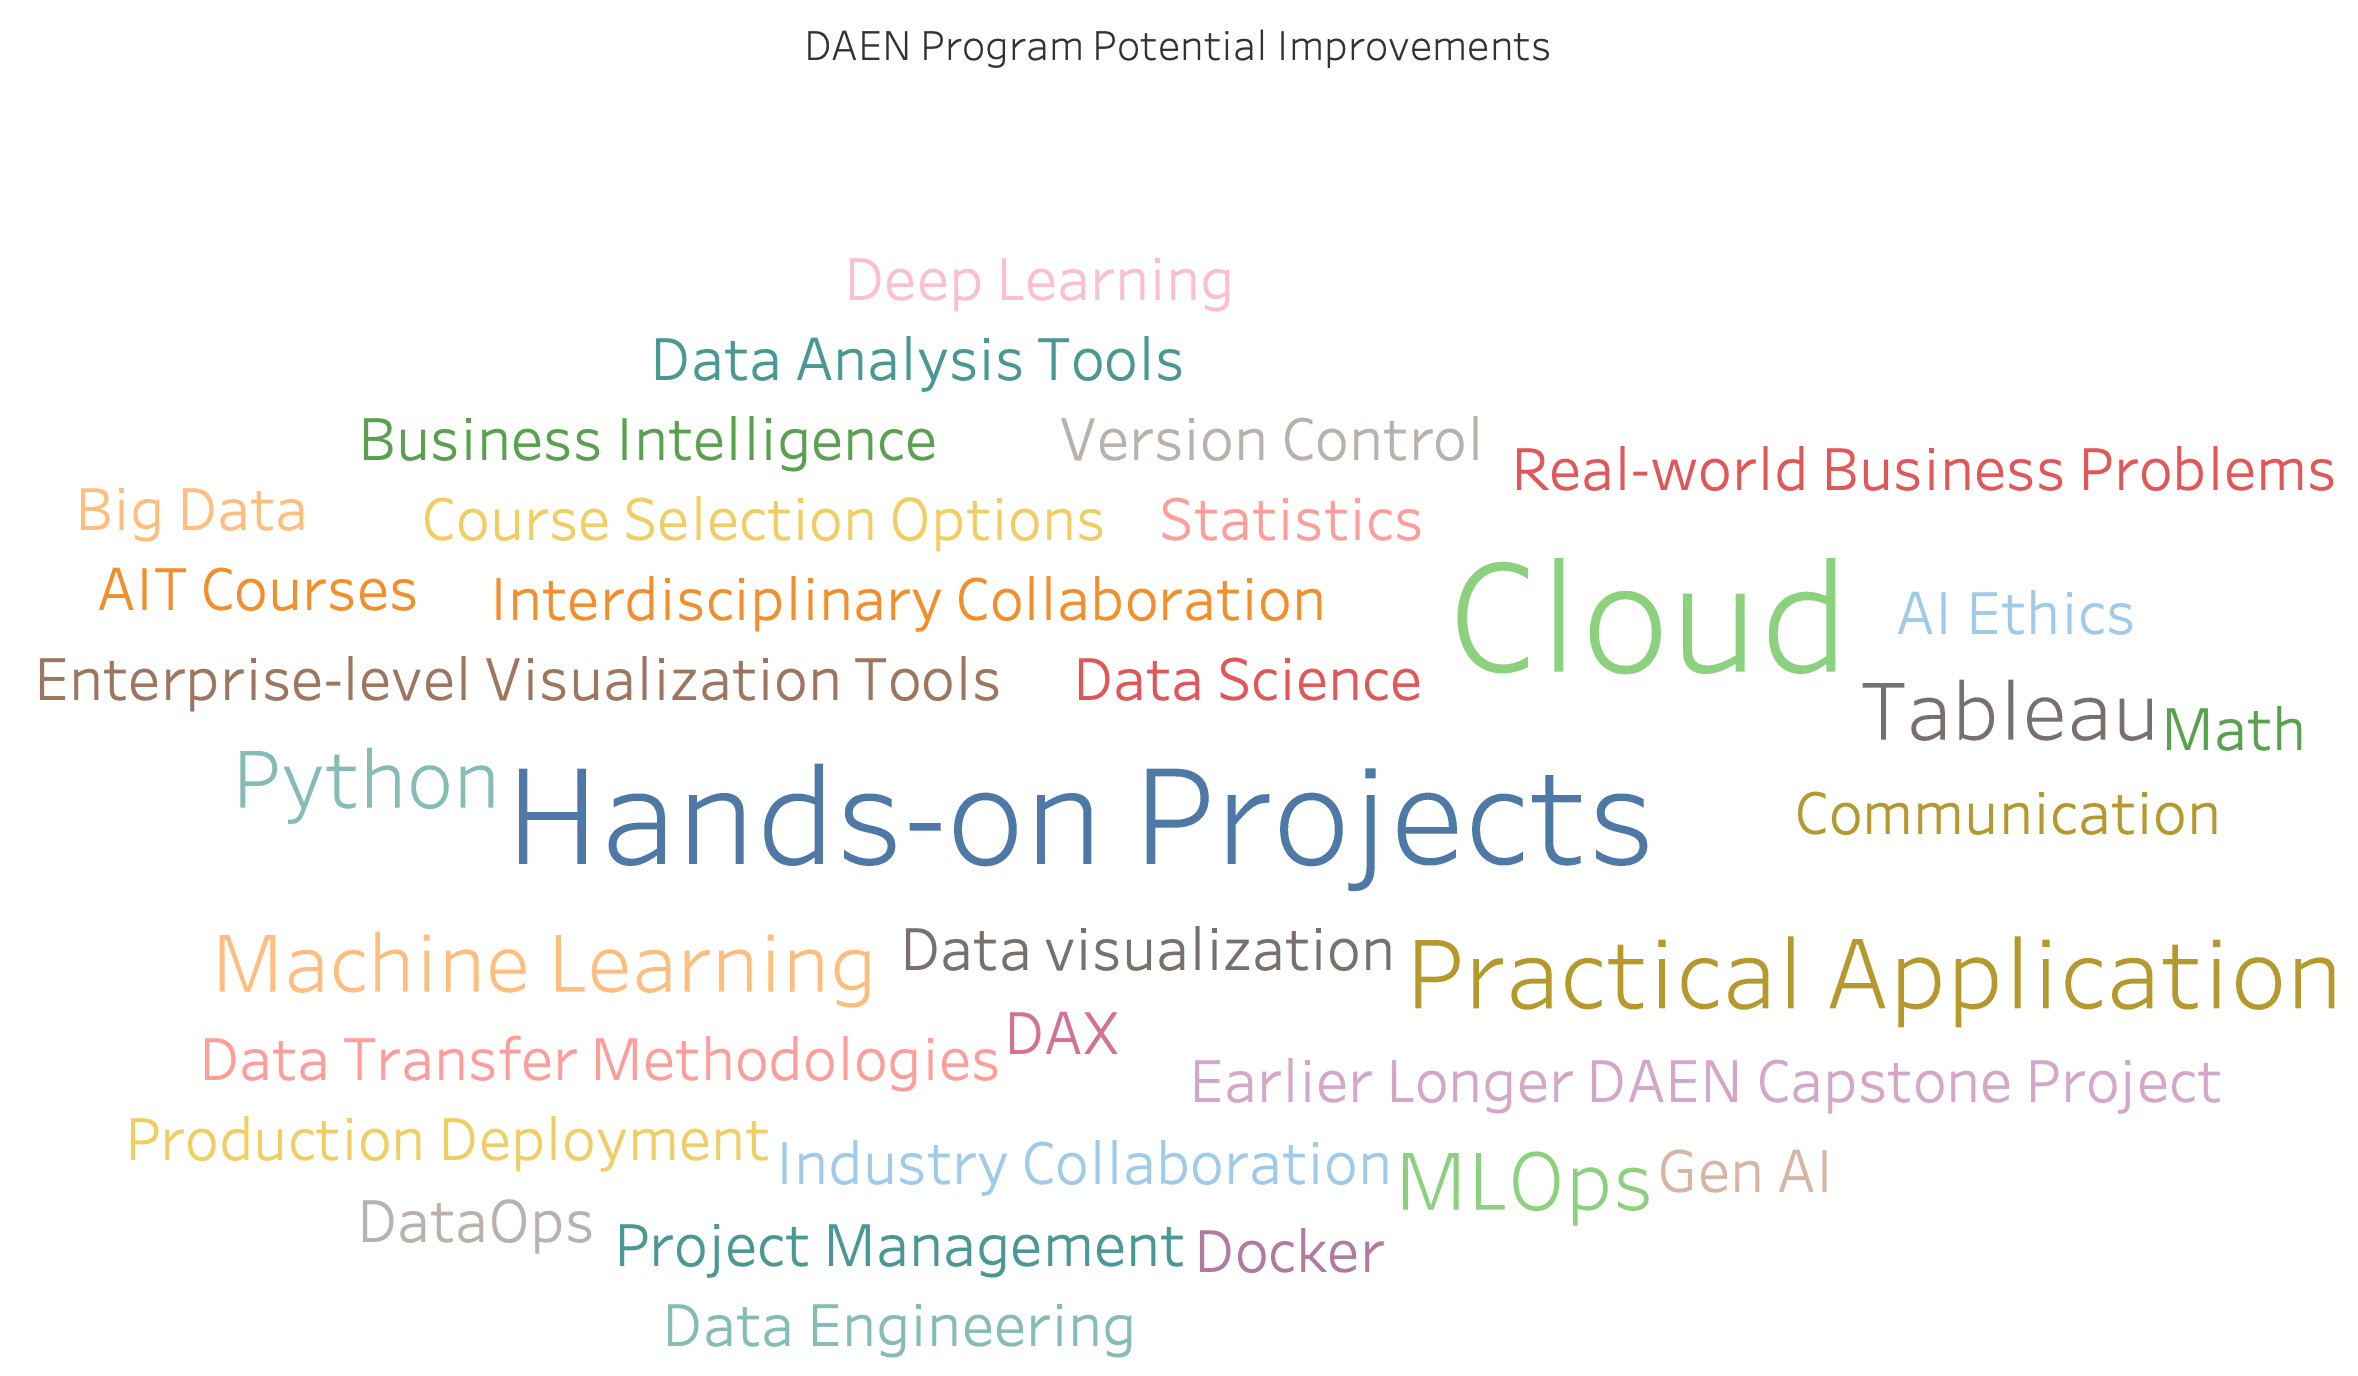
\includegraphics[width=0.9\textwidth]{visualizations/potential-improvements.png}
    \caption{Potential Program Improvements Suggested by Alumni}
    \label{fig:potential-improvements}
\end{figure}

\begin{figure}[H]
    \centering
    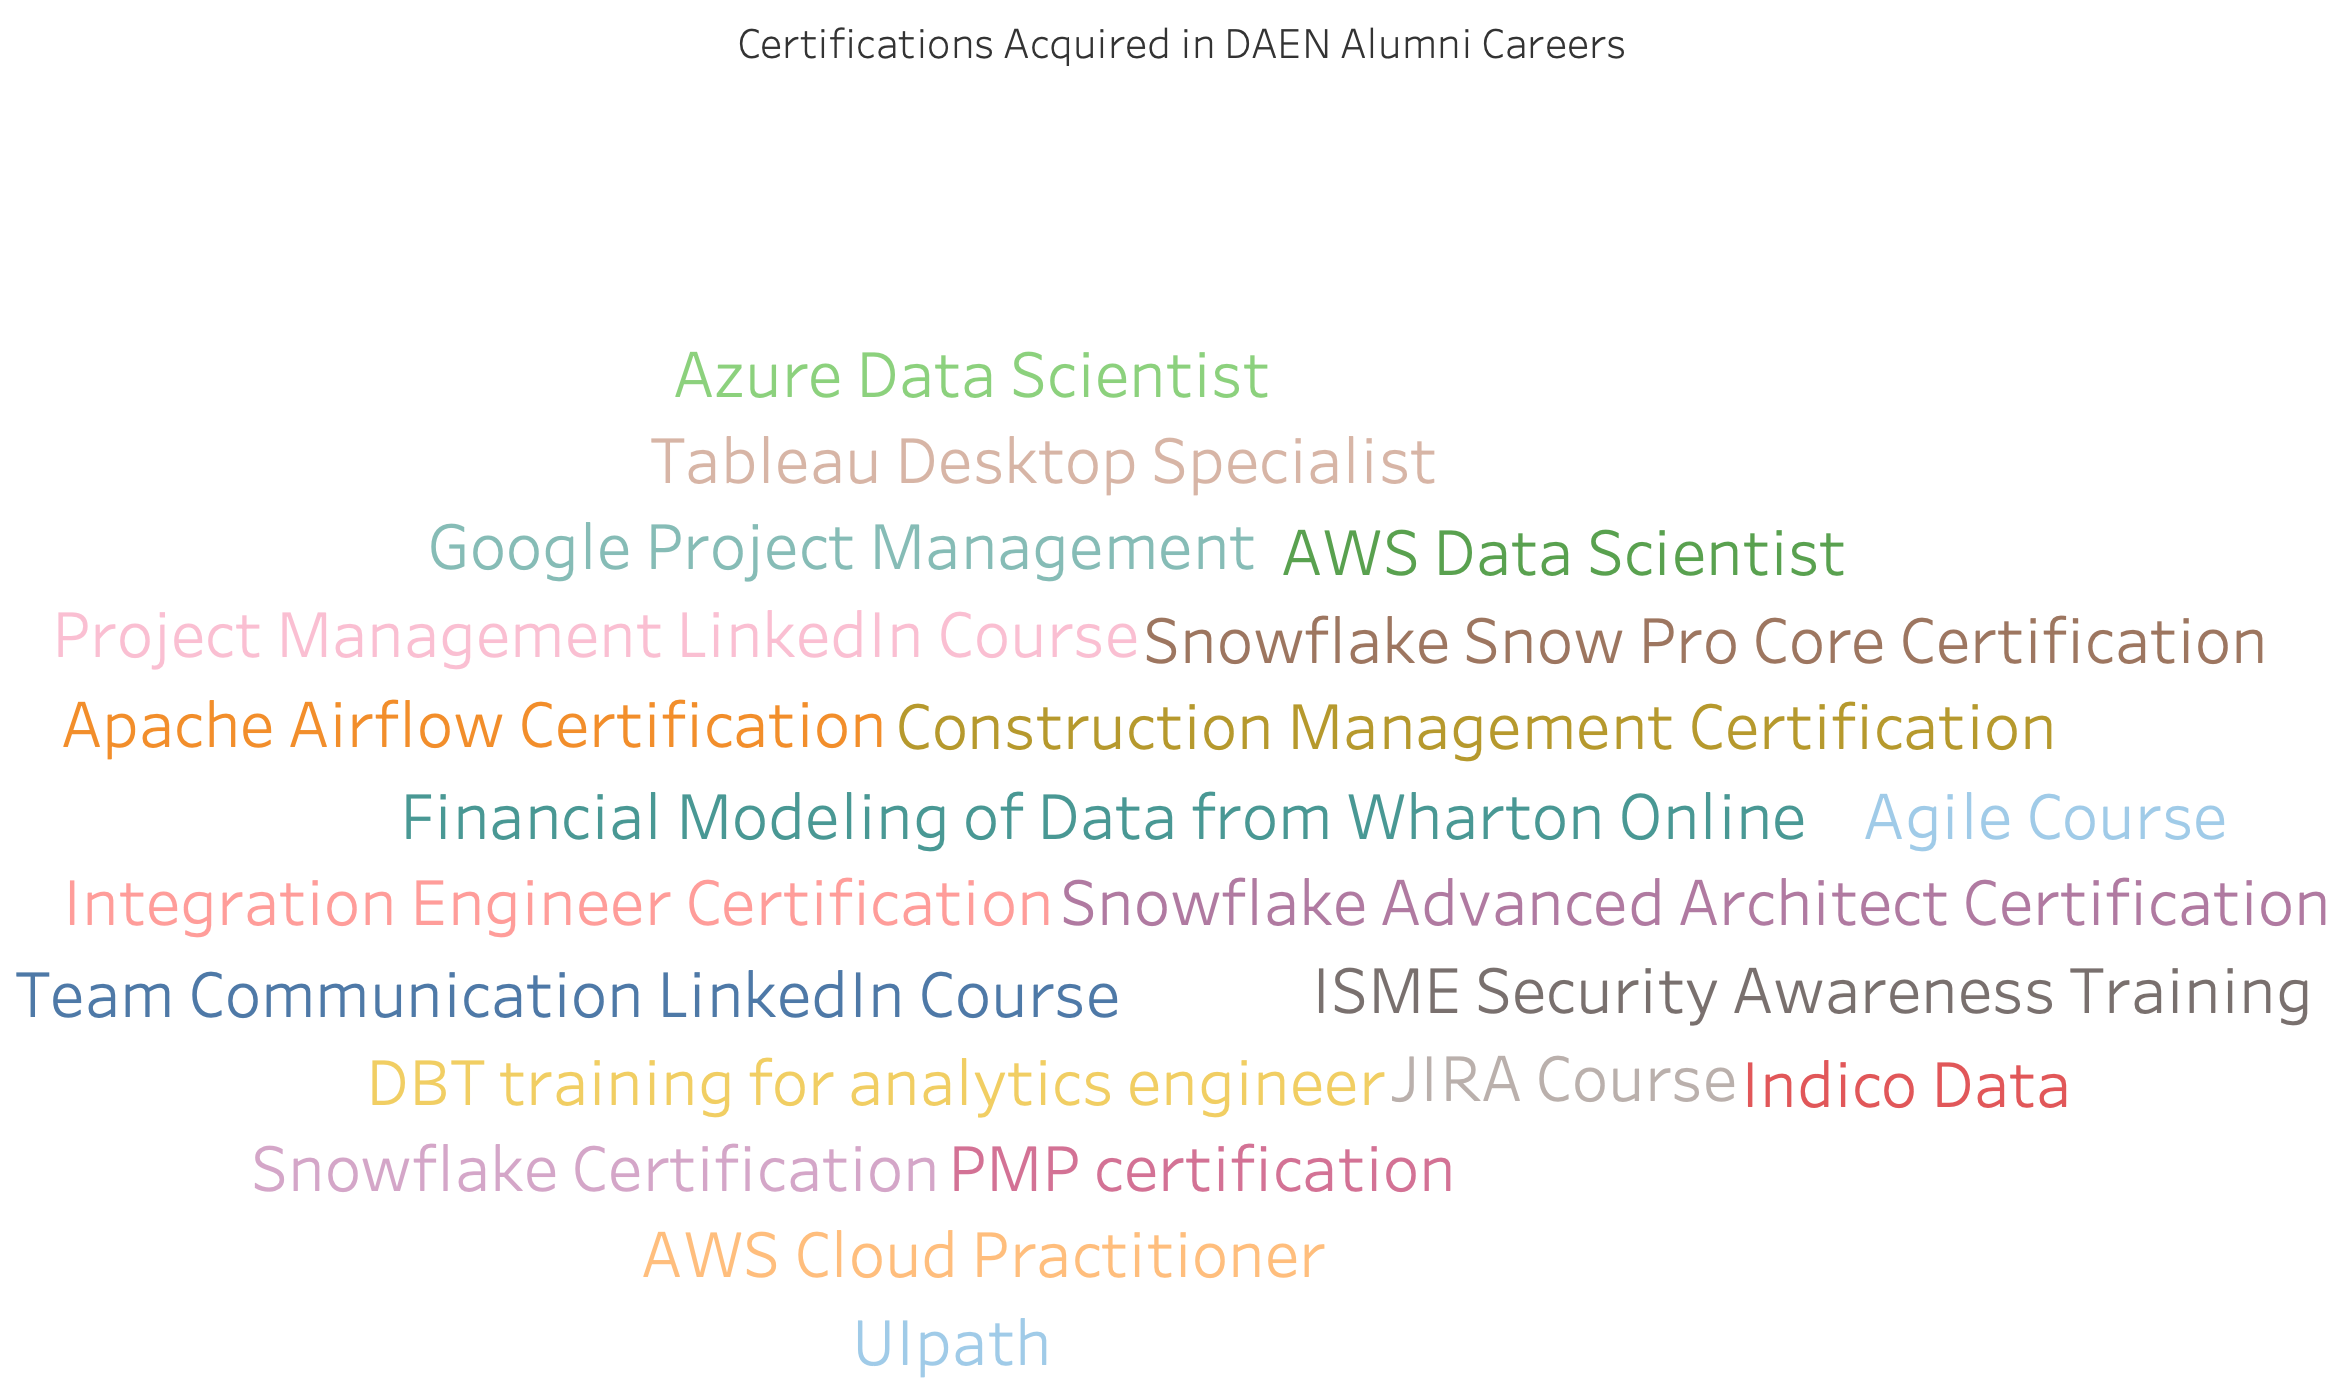
\includegraphics[width=0.9\textwidth]{visualizations/daen-alumni-completed-certs.png}
    \caption{DAEN Alumni Completed Certifications Post-Graduation}
    \label{fig:completed-certifications}
\end{figure}

% 6. Findings Section
\section{Findings}
Visualization analysis of interview data from 14 DAEN alumni provides comprehensive insights into the program's effectiveness and opportunities for curriculum enhancement. Among the participants, who graduated between 2019 and 2023, the largest cohort was from 2020 with five graduates. All participants completed their Master of Science degrees, representing a consistent focus on advanced education within the sample group.


Approximately 43\% of the alumni have held two jobs since graduation, indicating active career progression. Data Analyst emerged as the most common job category among DAEN alumni. DAEN alumni are employed across a diverse range of companies, with no dominant industry pattern emerging. The companies include major orgnizations and span various sectors, reflecting the program's broad applicability and industry recognition.


Technical skill utilization in alumni careers demonstrate clear trends in industry demands. SQL and Python rank as the most frequently utilized programming languages, aligning well with the program's educational emphasis, as these were also chosen as the most valuable technologies learned during the program. In terms of cloud technologies, AWS emerged as the dominant platform in professional settings, yet alumni suggest that cloud computing should be a key area for program improvement, as many received minimal cloud exposure during their studies. In the database domain, Snowflake has become the most widely used technology among graduates, complementing SQL and database systems which were ranked as the most valuable technology and tool acquired from the DAEN program. The alumni working with Snowflake have pursued professional certifications, including SnowPro Core and Advanced Architect credentials. Beyond traditional databases, graduates frequently utilize Spark and Databricks for Big Data processing and AI applications. Snowflake and Databricks are currently not covered in the DAEN program, indicating a potential implementation gap that could be addressed to enhance program relevance.


The program's effectiveness is reflected in its average rating of 3.7 out of 5, with the majority of alumni rating it 4 out of 5, indicating relatively high satisfaction with their education. DAEN 690 and Database courses are particularly highly valued by alumni, with machine learning and database systems highlighted as the most valuable tools acquired during the program. Data modeling and database skills were cited as crucial benefits of the program, demonstrating the curriculum's success in these areas.


Despite overall positive feedback, the analysis revealed several opportunities for program enhancement. Alumni consistently suggested increased emphasis on cloud computing technologies, particularly AWS, and recommended more hands-on project opportunities to bridge theoretical knowledge with practical application. There was also a clear desire for enhanced coverage of emerging technologies and methodologies, with a greater focus on practical, industry-relevant applications.


Post-graduation professional development patterns indicate ongoing learning needs in specific areas. Many alumni are pursing AWS certifications. While alumni pursue various professional certifications, there's no dominant pattern in their choices, as most certifications are completed based on specific job requirements and often sponsored by employers. This diversity in certification paths suggests an opportunity for the DAEN program to integrate specialized certification preparation into its curriculum, better aligning with industry demands and supporting graduates' career advancement.


% 7. Next Steps/Lessons Learned Section
\section{Next Steps and Lessons Learned}
\subsection{Next Steps}
The challenges encountered during this research highlighted the critical need for a systematic approach to alumni engagement. Beyond the initial hurdle of establishing contact, we discovered that motivating alumni to provide program-related feedback requires a well-designed outreach strategy. To ensure continuous program improvement, the department needs to implement a structured procedure for consistently collecting and analyzing alumni feedback. This systematic approach would not only streamline communication channels but also create a sustainable framework for gathering valuable insights about program effectiveness over time. Additionally, such a structured engagement system would enable the program to provide lifelong learning opportunities for alumni while staying current with industry demands. This ongoing connection would help maintain curriculum relevance and foster a strong sense of community that extends well beyond graduation.


Another critical lesson learned involves the design of survey questions to elicit more precise responses from alumni. During data collection, we observed that alumni often provided generalized answers due to the time elapsed since graduation, making it difficult to remember specific course details and experiences. These vague responses frequently had to be excluded from our analysis, reducing the overall quality of insights. Future surveys should strike a balance between collecting specific technical information and maintaining enough breadth to facilitate meaningful data categorization and analysis. This refined approach to question design would yield more actionable insights while enabling effective grouping of technologies, tools, and skills.


A streamlined approach to data processing is also essential for future research efforts. Our current data collection process revealed challenges with inconsistent interview recording formats, requiring individual handling of each case. While we utilized a local natural language processing toolkit for transcript extraction, a more robust design is needed to maximize information capture from interviews. Developing an automated processing pipeline would significantly improve the efficiency of analysis and visualization production. Time should be invested in establishing an optimal data analysis workflow that can handle diverse input formats while maintaining consistency in output generation.


Maintaining confidentiality of alumni information remains a paramount concern for future research. Survey and interview protocols should be carefully designed to exclude personal information while still gathering meaningful data. Creating a comfortable and secure interview environment is equally important, as it encourages alumni to provide candid feedback about their program experiences. This emphasis on privacy and comfort will help ensure the collection of honest, comprehensive insights that can genuinely contribute to program improvement.

\subsection{Lessons Learned}
Engaging alumni in program improvement initiatives presents a significant challenge, as graduates typically focus on their career progression and move forward from their academic experiences. The key to overcoming this challenge lies in implementing a systematic approach to alumni engagement, offering meaningful incentives for participation, and creating a comfortable interview environment that encourages open dialogue. Given that data collection emerged as the most challenging aspect of this research, future discussions should prioritize developing effective strategies for gathering alumni feedback. These strategies should acknowledge the time constraints and competing priorities that alumni face while still maintaining their involvement in program development.

% Appendices
\begin{appendices}
\section{Background}
This research, conducted as part of DAEN 698: Research Project, represents a significant initiative for both the program and department. As a pioneering effort in systematic alumni feedback collection, this study lays the groundwork for future program assessment and improvement. The insights gained from this initial research will catalyze further discussions and inspire continued investment in understanding and enhancing program effectiveness.

\section{References}
\begin{thebibliography}{9}
    \bibitem{gmu} George Mason University. (2024). Data Analytics Engineering, MS. Retrieved from https://catalog.gmu.edu/colleges-schools/engineering-computing/engineering/data-analytics-engineering-ms/
    \end{thebibliography}
\end{appendices}

\end{document}